%% This is file `elsarticle-template-1-num.tex',
%%
%% Copyright 2009 Elsevier Ltd
%%
%% This file is part of the 'Elsarticle Bundle'.
%% ---------------------------------------------
%%
%% It may be distributed under the conditions of the LaTeX Project Public
%% License, either version 1.2 of this license or (at your option) any
%% later version.  The latest version of this license is in
%%    http://www.latex-project.org/lppl.txt
%% and version 1.2 or later is part of all distributions of LaTeX
%% version 1999/12/01 or later.
%%
%% Template article for Elsevier's document class `elsarticle'
%% with numbered style bibliographic references
%%
%% $Id: elsarticle-template-1-num.tex 149 2009-10-08 05:01:15Z rishi $
%% $URL: http://lenova.river-valley.com/svn/elsbst/trunk/elsarticle-template-1-num.tex $
%%
\documentclass[preprint,12pt]{elsarticle}

%% Use the option review to obtain double line spacing
%% \documentclass[preprint,review,12pt]{elsarticle}

%% Use the options 1p,twocolumn; 3p; 3p,twocolumn; 5p; or 5p,twocolumn
%% for a journal layout:
%% \documentclass[final,1p,times]{elsarticle}
%% \documentclass[final,1p,times,twocolumn]{elsarticle}
%% \documentclass[final,3p,times]{elsarticle}
%% \documentclass[final,3p,times,twocolumn]{elsarticle}
%% \documentclass[final,5p,times]{elsarticle}
%% \documentclass[final,5p,times,twocolumn]{elsarticle}

%% The graphicx package provides the includegraphics command.
\usepackage{graphicx}
\usepackage{multicol}
\usepackage[poster=first]{animate}
\usepackage{subcaption}
\usepackage{caption}

%% The amssymb package provides various useful mathematical symbols
\usepackage{amssymb}
%% The amsthm package provides extended theorem environments
%% \usepackage{amsthm}

%% The lineno packages adds line numbers. Start line numbering with
%% \begin{linenumbers}, end it with \end{linenumbers}. Or switch it on
%% for the whole article with \linenumbers after \end{frontmatter}.
\usepackage{lineno}

%% The xcolor package is required to highlight table rows with 
%% different colors. 
\usepackage[table]{xcolor}
\usepackage{longtable}
\usepackage{multirow}
% Sideway figures and tables. 
\usepackage{rotating}
%% natbib.sty is loaded by default. However, natbib options can be
%% provided with \biboptions{...} command. Following options are
%% valid:

%%   round  -  round parentheses are used (default)
%%   square -  square brackets are used   [option]
%%   curly  -  curly braces are used      {option}
%%   angle  -  angle brackets are used    <option>
%%   semicolon  -  multiple citations separated by semi-colon
%%   colon  - same as semicolon, an earlier confusion
%%   comma  -  separated by comma
%%   numbers-  selects numerical citationsand
%%   super  -  numerical citations as superscripts
%%   sort   -  sorts multiple citations according to order in ref. list
%%   sort&compress   -  like sort, but also compresses numerical citations
%%   compress - compresses without sorting
%%
%% \biboptions{comma,round}

% \biboptions{}

\journal{Journal Name}

\begin{document}

\begin{frontmatter}

%% Title, authors and addresses

\title{Anticipating a fast transition from a concentrated to a generalized HIV epidemic in Madagascar} 
%% HIV transmission in  Madagascar: a dormant epidemic
%% neglected
%% use the tnoteref command within \title for footnotes;
%% use the tnotetext command for the associated footnote;
%% use the fnref command within \author or \address for footnotes;
%% use the fntext command for the associated footnote;
%% use the corref command within \author for corresponding author footnotes;
%% use the cortext command for the associated footnote;
%% use the ead command for the email address,
%% and the form \ead[url] for the home page:
%%
%% \title{Title\tnoteref{label1}}
%% \tnotetext[label1]{}
%% \author{Name\corref{cor1}\fnref{label2}}
%% \ead{email address}
%% \ead[url]{home page}
%% \fntext[label2]{}
%% \cortext[cor1]{}
%% \address{Address\fnref{label3}}
%% \fntext[label3]{}

%% use optional labels to link authors explicitly to addresses:
%% \author[label1,label2]{<author name>}
%% \address[label1]{<address>}
%% \address[label2]{<address>}

\author{David Alonso and Xavier Vall\`es}

% \address{Blanes, Barcelona, Catalonia}

\address{Computational and Theoretical Ecology Group \\ CEAB-CSIC, Blanes, Catalonia, Spain}

\begin{abstract}
With the widespread use of antiretroviral treatment and prevention measures, HIV incidence and AIDS related deaths have been declining in the last decade worldwide. However, most developing countries of the sub-Saharian region still experience a high burden of HIV/AIDS infection, specially in Southern and East Africa. Although Madagascar shares most risky factors for HIV  with surrounding countries, it has maintained an astonishing low levels of disease prevalence ($<$1\%). Here we develop a compartmental model to investigate the underlying reasons why this is so. Our approach allows for HIV prevalence projections in the different compartments up to year 2033 across most important cities in Madagascar, including biological, behavioural and demographic factors with special consideration of commercial sex  as a driver of HIV epidemic. We pointed to two hypothesis that could have delayed disease progression (cirumcision and/or late introduction). However, in spite of these plausible delaying factors, our model projections consistently predict that future HIV prevalence in Madagascar for 2030 might be significantly higher than current values (about 20-30\%), but probably stable and similar to other countries from the sub-Saharian region, unless urgent, strong control measures are set up focused on youth and people engaged on commercial sex. Our approach provides an additional quantitative tool to develop and test control strategies for HIV/AIDS in other countries as well.
\end{abstract}

\begin{keyword}
HIV/AIDS \sep Madagascar \sep sub-Saharian region \sep HIV/AIDS mathematical model \sep  SICA HIV/AIDS model \sep $R_0$ \sep circumcision \sep likelihood-based inferenece
%% keywords here, in the form: keyword \sep keyword
%% MSC codes here, in the form: \MSC code \sep code
%% or \MSC[2008] code \sep code (2000 is the default)
\end{keyword}

\end{frontmatter}

%%
%% Start line numbering here if you want
%%

\newpage

\linenumbers
%% main text
\section{Introduction}
\label{S:1}
The island of Madagascar (formally Republic of Madagascar) lies in the east coast of Africa, close to Mozambique and South-Africa, which experience a high burden of HIV/AIDS infection among General Population (GP), in spite of the steadily decrease of HIV incidence and AIDS related deaths since the widespread introduction of antiretroviral therapy (ART) in 2003 \cite{UNAIDS2019}. By contrast, Madagascar shows a very low prevalence of HIV in the GP ($<$1\%), alongside a high prevalence among the key populations (KP) for HIV spread: Men who have sex with Men (MSM), Sex workers (SW) and Injected Drug Users (IDU). This is an astonishing concentrated epidemic profile, particularly given that Madagascar shows a widespread presence of most of the most recognized risk factors associated to HIV acquisition in high prevalence countries \cite{Raberahona2020}. Since the late 90’s, previous articles have foreseen a close tipping point towards a generalized epidemic \cite{Behets2001,Raberahona2020}, which has not occurred to date, even if the general trend is an increase of prevalence among key populations (see \cite{Raberahona2020} and references therein). In this work, we develop a transmission disease model to address the question why Madagascar has not evolved to a generalized epidemic yet, and examine potential explanatory hypothesis of this peculiar situation, using biological, behavioural and demographic data available from this country. Mathematical models should be regarded as tools to explore this kind of questions in a quantitative way, producing estimates with controlled levels of uncertainty that may predict future disease progression and spread under various scenarios. Still, the modelling approach is frequently the only way to rise awareness and preparedness for plausible case-worse scenarios.
\smallskip
 
Initial mathematical models for HIV infection focused on the interaction between the immune system and the virus \cite{Nowak01,Keeling08}. More recently, several models have been developed to analyze the transmission dynamics of the disease in a population \cite{Mukandarive2007,MUKANDAVIRE2009,Kim2014,Aldila2018,Omondi2018,Omondi2019}, and some of them have already included age and sex structure \cite{Mukandarive2007,Omondi2018,Omondi2019}. The model we present in this article takes a step further and, in addition to include well-established biological data about HIV transmission, it is grounded on sound demographic data and partial behavioural knowledge from Madagascar population. This involves considering necessary, but plausible assumptions, which will be thoroughly discussed.  Furthermore, we pay attention to the particularities of Madagascar, like the widespread practice of circumcision. Indeed, our model considers separately the ten most important cities in Madagascar (Antananarivo, Toamasina, Mahjanga, Nosy Be, Antsiranana, Moramanga, Morondava, Fianarantsoa, Toliary and Toalagnaro) from which basic data are available. 
 \smallskip

 In the following sections, we will carefully introduce the "{\bf S}usceptible-Acute {\bf I}nfected-{\bf C}hronic Infected-{\bf A}IDS phase infected" transmission model ({\bf $SICA$}), estimate model $R_0$ for several cities in 2000 when disease levels were probably very low, and demonstrate how to incorporate in our analyses all demographic, hehavioural, and disease information available to date for Madagascar. Here we address why Madagascar still shows this low HIV epidemic profile, but the SICA model could be a valuable tool to monitor HIV epidemic and better address interventions to control it elsewhere. 

\section{Materials and Methods}
\subsection{$SICA$ Transmission Model}
We represent the temporal dynamics of disease spread by a set of ordinary differential equations \cite{Anderson91}. This system represents the progression of the disease as a consequence of sexual encounters between infectious and non-infected individuals. The whole population is divided in a set of groups. Male population is considered as a single group, while female population is subdivided into four groups: two groups according to sexual activity (sexual workers and rest of women), where each of them is in turn subdivided into young (15 to 25 years old) and adult females. Both males and females are recruited into the population as fully susceptible individuals, represented by the subscript $S$ in the set of dynamic variables ---see Eqs (\ref{eq:Y})-(\ref{eq:W_1}). These recruitment rates are defined as the number of males and females per unit time that reach sexual maturity at any given time. As these individuals encounter infectious sexual partners, they can acquire the virus and then transition to the HIV acute infection stage (see subscript $I$ in the equations below). This stage lasts, on average, between 2 and 3 months \cite{Fiebig2003,Hollingsworth2008} (see $\gamma$ values in Table \ref{T1:Parameter_Values}), and is characterized by a transient high viral load (Fig \ref{Fig:1}), and, as a result, individuals are ten to hundred times as infectious as during the following phase, the chronic phase \cite{Pinkerton2008,Hollingsworth2008}. After this first acute phase, individuals transition into a clinically stable, chronic stage, where they are characterized by lower viral loads. The duration of this second phase (see subscript $C$) is controlled by rate $\mu$, and lasts around 10 years \cite{Bacchetti1989,Hollingsworth2008}, followed by the breakdown of their immune system. When this occurs, individuals enter a terminal stage (Acquired Immunodeficiency Disease Syndrome or AIDS stage) (see subscript $A$) where most disease-induced mortality concentrates if no treatment is provided (see Fig \ref{Fig:1}). 
\smallskip

\begin{figure}
\centering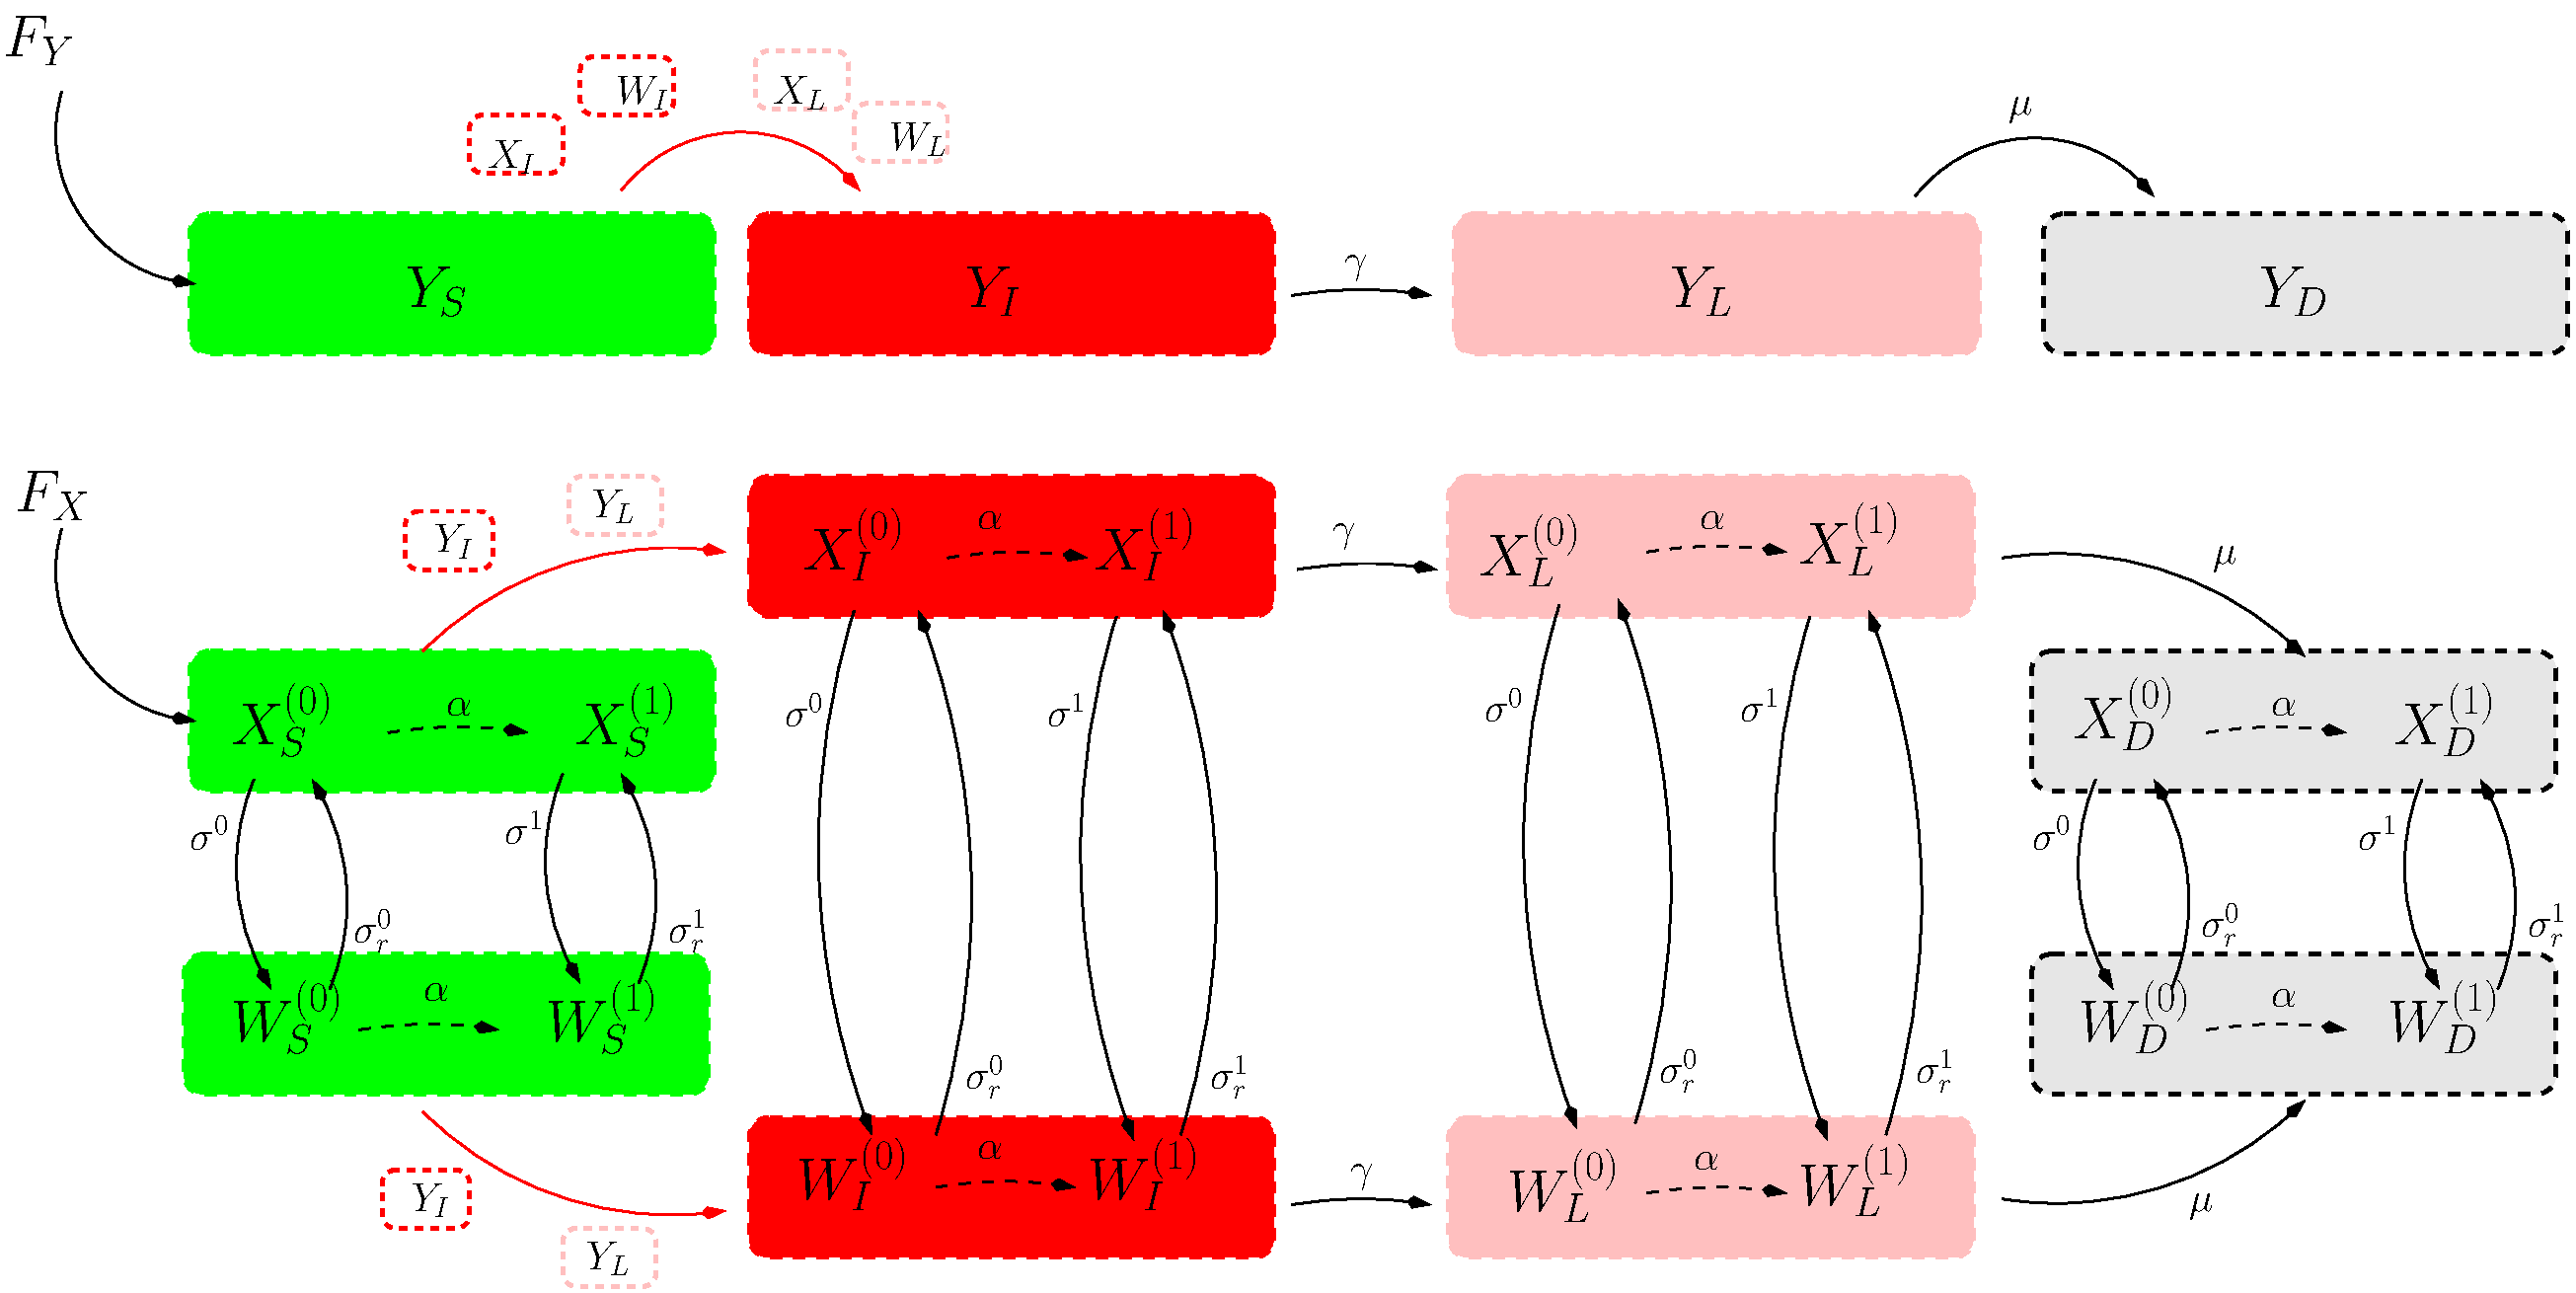
\includegraphics[width=1.0\linewidth,angle=0]{HIV_Fig1_Full}
\caption{\label{Fig:1} Graphic representation of women and men subpopulations progressing through the different stages of the disease since they acquire the infection from infectious males ($Y_I$ or $Y_C$) and women ($\hat{X}_I$, $\hat{X}_C$), respectively. At any stage of the disease, women can become sexual workers, at rate $\sigma$, or reverse that condition, at rate $\sigma_r$. The {\em aging} rate $\alpha$ controls the transition from young to adult women. All stages, both in men and women, are subject to mortality. For simplicity, arrows representing this fatal transition are not shown.}
\end{figure}

The female-male coupled system is then organized into the male and the female submodels. These separate submodels are coupled through the force of infection or transmission rate, this is, the per capita rate at which male (or female) susceptible individuals acquire the infection through sexual contacts from female (or male) infectious individuals. This transmission rate takes into account the number of sexual contacts per year of an average male (or female) individuals, $\beta_Y$ (or $\beta_X$), the distinct probability of transmission from infectious females to males (or from infectious males to females) \cite{Hollingsworth2008}, $p_{YX}$ (or $p_{XY}$), and the effective population fractions of infectious females (or males), $x$ (or $y$) \cite{McCallum2001}. Notice also that basal female contact rate, $\beta_X$, is corrected by a factor $\eta > 1$ for sexual workers to indicate the higher contact rates characterizing this activity. 
\smallskip

The male subsystem reads:
\begin{eqnarray}
\frac{dY_S}{dt} & = & F_Y - \beta_Y\,p_{YX}\,x\, Y_S - \delta\,Y_S \nonumber\\
%\label{eq:Y_S}
\frac{dY_I}{dt} & = & \beta_Y\,p_{YX}\,x\, Y_S - \delta\,Y_I -\gamma\,Y_I \nonumber\\
%\label{eq:Y_I}
\frac{dY_C}{dt} & = & \gamma\,Y_I - \mu\, Y_C  - \delta\,Y_C \nonumber\\
%\label{eq:Y_C}
\frac{dY_A}{dt} & = & \mu\, Y_C - (1+m)\,\delta\, Y_A
%\label{eq:Y_A}
\label{eq:Y}
\end{eqnarray}
where the total effective fraction of infectious females is a weighted average of the effective infectious fractions including young, $x_0$, and adult women, $x_1$:
\begin{equation}
x = f_0\, x_0 + (1-f_0)\,x_1
\label{eq:x_fraction}
\end{equation}
where $f_0$ is the fraction of total sexual encounters a male has with young females. Effective infectious fractions of females should account for differential transmission of the disease from females either in the highly infectious group or the chronic group:
\begin{equation}
x_0 = \frac{ f_W\,(\chi\,W^{(0)}_I+W^{(0)}_C) + (1-f_W)(\chi\,X^{(0)}_I+X^{(0)}_C) }{N_f}
\label{eq:x0_fraction}
\end{equation}
\begin{equation}
x_1 = \frac{ f_W\,(\chi\,W^{(1)}_I+W^{(1)}_C) + (1-f_W)(\chi\,X^{(1)}_I+X^{(1)}_C) }{N_f}
\label{eq:x1_fraction}    
\end{equation}
where $f_W$ if the fraction of male sexual contacts with women who are sexual workers, and $N_f$ is the total female population. 
\smallskip

The female subsystem accounts for the progression of the disease in the four female groups, which all follow the same four-equation scheme. Equations for young females that are not non-sexual workers are given by:
\begin{eqnarray}
\frac{dX^{(0)}_S}{dt} & = & F_X - \beta_X\,p_{XY}\,y\, X^{(0)}_S - \delta\,X^{(0)}_S -\alpha \, X^{(0)}_S - \sigma^0\,X^{(0)}_S + \sigma^0_r\,W^{(0)}_S\nonumber\\
\frac{dX^{(0)}_I}{dt} & = & \beta_X\,p_{XY}\,y\, X^{(0)}_S - \delta\,X^{(0)}_I -\alpha \, X^{(0)}_I - \gamma\,X^{(0)}_I -\sigma^0\,X^{(0)}_I + \sigma^0_r\,W^{(0)}_I\nonumber\\
\frac{dX^{(0)}_C}{dt} & = & \gamma\,X^{(0)}_I - \mu\, X^{(0)}_C  - \delta\,X^{(0)}_C -\alpha \, X^{(0)}_C - \sigma^0\,X^{(0)}_C + \sigma^0_r\,W^{(0)}_C\nonumber\\
\frac{dX^{(0)}_A}{dt} & = & \mu\, X^{(0)}_C - (1+m)\,\delta\, X^{(0)}_A -\alpha \, X^{(0)}_A - \sigma^0\,X^{(0)}_A + \sigma^0_r\,W^{(0)}_A
\label{eq:X_0}
\end{eqnarray}
\smallskip

The four basic equations for old/adult non-sexual-worker females are:
\begin{eqnarray}
\frac{dX^{(1)}_S}{dt} & = & - \beta_X\,p_{XY}\,y\, X^{(1)}_S - \delta\,X^{(1)}_S + \alpha \, X^{(0)}_S -\sigma^1\,X^{(1)}_S + \sigma^1_r\,W^{(1)}_S\nonumber\\
\frac{dX^{(1)}_I}{dt} & = & \beta_X\,p_{XY}\,y\, X^{(1)}_S - \delta\,X^{(1)}_I + \alpha\,X^{(0)}_I - \gamma\,X^{(0)}_I -\sigma^1\,X^{(1)}_I + \sigma^1_r\,W^{(1)}_I\nonumber\\
\frac{dX^{(1)}_C}{dt} & = & \gamma\,X^{(1)}_I - \mu\, X^{(1)}_C  - \delta\,X^{(1)}_C + \alpha\,X^{(0)}_C - \sigma^1\,X^{(1)}_C + \sigma^1_r\,W^{(1)}_C\nonumber\\
\frac{dX^{(1)}_A}{dt} & = & \mu\, X^{(1)}_C - (1+m)\,\delta\, X^{(1)}_A + \alpha\,X^{(0)}_A - \sigma^1\,X^{(1)}_A + \sigma^1_r\,W^{(1)}_A
\label{eq:X_1}
\end{eqnarray}
\smallskip

Likewise, the four equations for young, sexual-worker females read:
\begin{eqnarray}
\frac{dW^{(0)}_S}{dt} & = & - \beta_X\,p_{XY}\,(1+\eta)\,y\, W^{(0)}_S - \delta\,W^{(0)}_S -\alpha \, W^{(0)}_S - \sigma^0_r\,W^{(0)}_S + \sigma^0\,X^{(0)}_S\nonumber\\
\frac{dW^{(0)}_I}{dt} & = & \beta_X\,p_{XY}\,(1+\eta)\,y\, W^{(0)}_S - \delta\,W^{(0)}_I -\alpha \, W^{(0)}_I -\gamma\,W^{(0)}_I -\sigma^0_r\,W^{(0)}_I + \sigma^0\,X^{(0)}_I\nonumber\\
\frac{dW^{(0)}_C}{dt} & = & \gamma\,W^{(0)}_I - \mu\, W^{(0)}_C  - \delta\,W^{(0)}_C - \alpha \, W^{(0)}_C - \sigma^0_r\,W^{(0)}_C + \sigma^0\,X^{(0)}_C\nonumber\\
\frac{dW^{(0)}_A}{dt} & = & \mu\, W^{(0)}_C - (1+m)\,\delta\, W^{(0)}_A -\alpha \,W^{(0)}_A - \sigma^0_r\,W^{(0)}_A + \sigma^0\,X^{(0)}_A
\label{eq:W_0}
\end{eqnarray}
\smallskip

Finally, the equations for old/adult sexual-worker females are represented by:
\begin{eqnarray}
\frac{dW^{(1)}_S}{dt} & = & - \beta_X\,p_{XY}\,(1+\eta)\,y\, W^{(1)}_S - \delta\,W^{(1)}_S + \alpha \, W^{(0)}_S-\sigma^1_r\,W^{(1)}_S + \sigma^1\,X^{(1)}_S\nonumber\\
\frac{dW^{(1)}_I}{dt} & = & \beta_X\,p_{XY}\,(1+\eta)\,y\, W^{(1)}_S - \delta\,W^{(1)}_I + \alpha \, W^{(0)}_I -\gamma\,W^{(1)}_I -\sigma^1_r\,W^{(1)}_I + \sigma^1\,X^{(1)}_I\nonumber\\
\frac{dW^{(1)}_C}{dt} & = & \gamma\,W^{(1)}_I - \mu\, W^{(1)}_C  - \delta\,W^{(1)}_C + \alpha \, W^{(0)}_C - \sigma^1_r\,W^{(1)}_C + \sigma^1\,X^{(1)}_C\nonumber\\
\frac{dW^{(1)}_A}{dt} & = & \mu\, W^{(1)}_C - (1+m)\,\delta\, W^{(1)}_A + \alpha \,W^{(0)}_A - \sigma^1_r\,W^{(1)}_A + \sigma^1\,X^{(1)}_A
\label{eq:W_1}
\end{eqnarray}
\smallskip

As you see in Eqs (\ref{eq:X_0})-(\ref{eq:W_1}), the force of infection of females includes a factor, the total effective fraction of infectious males, $y$, which is given by:
\begin{equation}
y = \frac{\chi\,Y_I + Y_C}{N_m}
\label{eq:y}
\end{equation}
where $N_m$ is the total male population. Total populations, $N_m$ and $N_f$, also change dynamically. They are written in terms of sums over the different disease stages and groups:
\begin{eqnarray}
N_m & = & Y_S + Y_I + Y_C + Y_A                        \nonumber\\
N_f & = & \hat{X}_S + \hat{X}_I + \hat{X}_C + \hat{X}_A
\label{eq:N}
\end{eqnarray}
where
\begin{eqnarray}
  	\hat{X}_a & = & X^{(0)}_a + X^{(1)}_a + W^{(0)}_a + W^{(1)}_a \nonumber\\
	        a & \in & \{{\tiny S, I, C, A}\} 
	\label{eq:X_hat}
\end{eqnarray}

Total effective infectious fractions, $x$ an $y$, are the link between female and male disease dynamics. These parameters are not constrained between 0 and 1 because they include the factor $\chi > 1$, which measures the increase in transmission of infectious individuals in the acute phase compared to the chronic phase (they would be only proper fractions if $\chi$ were 1). In any case, these parameters times $p_{XY}$ (or $p_{YX}$) determine the probability rate of acquiring the infection per sexual encounter. The rest of symbols appearing in the equations are explained in Table \ref{T1:Parameter_Values}.

\hspace{-1.0cm}\begin{table}
% \rowcolors{1}{green}{pink}
% \rowcolors{1}{blue!15}{white}
\centering
\begin{tabular}{p{7.0cm}ccccc}
{\bf Model Parameter}                                  & {\bf Symbol}   & {\bf $V_0$} & {\bf $V_1$} & {\bf Refs.}\\
\hline\hline
\rowcolor{blue!15}              % Heading with different color to highlight it
\multicolumn{5}{c}{Demographic parameters}\\
\hline
{\small Recruitment rate into active sexual age}        & $F_Y$         & 0.00 & 5 10$^4$ & \cite{webSexRatio}\\
{\small Recruitment rate into active sexual age}        & $F_X$         & 0.00 & 5 10$^4$ & \cite{webSexRatio}\\
{\small Natural mortality percapita rate (X)}           & $\delta_X$    & 0.01 & 0.05     & \cite{webSexRatio}\\
{\small Natural mortality percapita rate (Y)}           & $\delta_Y$    & 0.01 & 0.05     & \cite{webSexRatio}\\
{\small Aging rate into the AF stage}                   & $\alpha$      & 0.08 & 0.12     & \\  
{\small Transition rate into the SW stage (YF)}         & $\sigma^0$    & 0.00 & 0.05     & \\
{\small Reverse rate from the SW stage (YF)}            & $\sigma^0_r$  & 0.00 & 0.05     & \\
{\small Transition rate into the SW stage (AF)}         & $\sigma^1$    & 0.00 & 0.05     & \\
{\small Reverse rate from the SW stage (AF)}            & $\sigma^1_r$  & 0.00 & 0.05     & \\
\hline
\rowcolor{pink}              % Heading with different color to highlight it
\hline
\multicolumn{5}{c}{Disease transmission parameters}\\
\hline
{\small Total male sexual contact rate}                    & $\beta_Y$   & 96.0 & 120.0   &  \cite{Wawer2005}\\
{\small Total female sexual contact rate}                  & $\beta_X$   & 96.0 & 120.0   &  \cite{Wawer2005}\\
{\small Sexual worker $\beta_X$ factor [$(1+\eta)\beta_X$}] & $\eta$      & 0.00 & 19.00  & \\
{\small Male-to-Female transmission probability}           & $p_{XY}$    & 0.00 & 0.005   & \cite{Patel2014,Wawer2005,Gray2001}\\
{\small Female-to-Male transmission probability}           & $p_{YX}$    & 0.00 & 0.001   & \cite{Patel2014,Wawer2005,Gray2001} \\  
{\small Transition rate from $I$ into $C$ stage}           & $\gamma$    & 0.5  & 6.00    & \cite{Fiebig2003}\\
{\small Transition rate from $C$ into $A$ stage}           & $\mu$       & 0.05 & 0.20    & \cite{Bacchetti1989}\\
%{\small Number of substages during $L$ phase}              & $n$         & 1.00 & 10.00 & 1.00\\
{\small Disease-induced mortality factor [$(1+m)\delta$}]   & $m$         & 0.00 & 99.00   & \\ 
{\small Infectious phase ($I$) transmission factor}        & $\chi$      & 1.00 & 100.00   & \cite{Pinkerton2008}\\
{\small Male sexual preference factor (for SW)}            & $f_W$       & 0.00 & 0.99     & \\
{\small Male sexual preference factor (for YF)}            & $f_0$       & 0.00 & 0.99     & \\
\hline\hline
\end{tabular}
\caption{Model Parameters for the $SICA$ model. $V_0$ and $V_1$ define reasonable parameter ranges for each parameter value. Subscripts X and Y stand for female and male, respectively. YF, young female; AF, adult female; SW, sexual worker. All rates are given in year$^{-1}$. Mortality and recruitment rates are directly estimated from life table information. Transmission probabilities are given per coital act and represent basal values. The $\chi$ factor controls how much these are incremented when a healthy individual has a sexual encounter with an individual in the acute infection phase ($I$). The inverse of transition rates between stages (for instance, $1/\gamma$ and $1/\mu$) can be regarded as an average residence time in that stage, respectively). Consequently, the range for the average length of the infection phase ($I$) (see $\gamma$ values) is considered to be between 2 months and 2 years (an average of 70 days after \cite{Fiebig2003}). Likewise, the average length of the $C$ phase (see $\mu$ values) may span from 5 to 20 years (an average of 9.8 years after \cite{Bacchetti1989}), and the average duration of a young age for females (see $\alpha$ values) is considered to be between 8 and 12 years after entering full active sexual life (at the age of 15).}
\label{T1:Parameter_Values}
% Parameter $n$ determines de variance of the distribution for the residence time in the $L$ phase.
\end{table}

\subsection{Demographic Model}
% \subsubsection{Model assumptions}
The SILD model extremely simplifies population demography. In the absence of disease transmission, once can check that female and male subpopulations evolve in time according to the following system:
\begin{eqnarray}
\frac{dY}{dt} & = & F_Y - \delta_Y Y \nonumber\\
\frac{dX^{(0)}}{dt} & = & F_X -\sigma^0 X^{(0)} +\sigma_r^0 W^{(0)} -\alpha X^{(0)} -\delta_X X^{(0)} \nonumber\\
\frac{dW^{(0)}}{dt} & = & \sigma^0 X^{(0)} -\sigma_r^0 W^{(0)} -\alpha W^{(0)} -\delta_X W^{(0)} \nonumber \\
\frac{dX^{(1)}}{dt} & = & \alpha X^{(0)} + \sigma_r^0 W^{(1)} -\sigma^0 X^{(1)} -\delta_X X^{(1)} \nonumber\\
\frac{dW^{(1)}}{dt} & = & \alpha W^{(0)} + \sigma^0 X^{(1)}  -\sigma_r^0 W^{(1)} -\delta_X W^{(1)}
\label{Eq:Demography_0}
\end{eqnarray}

Further simplification is reached if we sum up over female equations. Female and male adult populations are just tracked by the simple system:
\begin{eqnarray}
\frac{dY}{dt} & = & F_Y - \delta_Y \, Y\nonumber\\
\frac{dX}{dt} & = & F_X - \delta_X \, X
\label{Eq:Demography_S}
\end{eqnarray}

Importantly, demographic trends are reflected in parameter values changing from year to year. Realistically, demographic parameters evolve in time. Adult populations are driven by temporal-dependent demographic parameters (recruitment rates, $F_X$ and $F_Y$, and adult mortality rates, $\delta_X$ and $\delta_Y$). $F_X$ and $F_Y$ represent the absolute number of females and males entering sexual active life per year, respectively. They depend on the population size of every city and, due to demographic growth (and, probably, immigration), have a monotone increase with time. In the supplementary information, we explain the strategy we followed to accurately estimate them from demographic life table data. 
\smallskip

The rest of model demographic parameters ($\alpha$ and $\sigma$'s) were searched to be compatible with surveyed SW population across cities in 2014 and 2017. Since this can be done in infinite different ways, we chose to fit a trajectory for the number of sexual workers that could have been observed from 2000 to 2016 under two reasonable hypotheses, namely, the {\em constant-fraction} and the {\em sigmoidal} hypotheses. The first one assumes that the average fraction of SW in the population remained constant over the whole period of interest (2000-2016). The second hypothesis takes into consideration Madagascar economic crises (2009-2013) and makes the assumption that the fraction of sexual workers within the adult female population could have increased as a consequence of the crisis. We modeled this growth as a sigmoidal curve (see Supp Mat for details).  

\subsection{Realistic Model Projections}
Temporal evolution of HIV prevalence for every key group can be calculated by numerical integrating the full ODE system (see Eqs. (\ref{eq:Y}), (\ref{eq:X_0})-(\ref{eq:W_1}), and the definitions of the infectious effective fractions, $x$ and $y$, given by Eqs. (\ref{eq:x_fraction})-(\ref{eq:x1_fraction}), and (\ref{eq:y}),  and total populations as given by Eqs (\ref{eq:N})-(\ref{eq:X_hat})). However, only when we let parameters annually change according to data, we obtain a realistic demographic trajectory. Predictions for disease spread in the different groups can then be generated by numerically integration of the system considering that demographic key parameters are no longer constant but change annually. 
\smallskip

Parameter estimations were based on several data sources \cite{DataSourceCIA2018,DataSourceWHO2018,DataSourceInstat-Madagascar2018,DataSourceWM2019}. Initial population values were chosen to correspond to the year 2000. Adult sex ratio is considered 1:1 \cite{webSexRatio,DataSourceWHO2018}.  
Disease initial prevalence for sexual workers was set to be a 1\% of prevalence value for each city in 2016 (see Table \ref{Table:Madagascar_Cities}). These yields very low initial numbers of infected individuals in 2000 (between 1 and 10 for most cities). Disease prevalence for the rest of groups at the initial year are then set accordingly. Model projections are then calculated from 2016 up to year 2033 taking into account the uncertainty we have in model parameter estimates, and assuming that demographic age-specific {\em per capita} rates follow the overall trend of the period 2000-2016 (see Supp Mat). 

% Discussio: Other scenarios can also be explored? 
% either (A) they do not change on average significantly or (B) they follow the overall trend of the period 2000-2016

% (\ref{eq:X_1})-(\ref{eq:W_0})
\begin{sidewaystable}
\caption{Total and sexual worker population and prevalence within this group for the main cities in Madagascar. Source: Institut National de la Statistique, Antananarivo.}
\bigskip
% \rowcolors{1}{green}{pink}
% \rowcolors{1}{blue!15}{white}
\centering
\begin{tabular}{crrrrrcccccc}
\hline
\hline
\rowcolor{blue!15}  
        & Population & \multicolumn{4}{c}{Sexual Worker Population} & \multicolumn{6}{c}{HIV Prevalence} \\
\rowcolor{blue!15}  
        & 2013       & \multicolumn{2}{c}{2014} & \multicolumn{2}{c}{2017} & \multicolumn{3}{c}{2012} & \multicolumn{3}{c}{2016} \\
\rowcolor{blue!15}  
        &            & {\small Min} & {\small Max} & {\small Min} & {\small Max}& \% & \multicolumn{2}{c}{\small CI} & \% & \multicolumn{2}{c}{\small CI}\\
\hline
Antananarivo  & 1300000 & 28925 & 35021 & 4908	& 12647 & 0.2  & 0.0  & 0.6  & 1.8  & 0.4  & 4    \\ 
Antsiranana   & 115015  & 2978  & 6812  & 4489	& 10749 & 0.0  & 0.0  & 0.0  & 2.9  & 0.8  & 6.5  \\
Mahajanga     & 220629  & 2290  & 5637  & 571	& 1516  & 3.0  & 0.8  & 6.2  & 22.7 & 13.9 & 31.2 \\ 
Toamasina     & 274667  & 4289  & 12336 & 3638	& 15120 & 1.8  & 0.2  & 3.9  & 5.4  & 2.9  & 8.1  \\
Fianarantsoa  & 190318  & 3415  & 7795  & 743	& 2961  & 0.9  & 0.0  & 1.4  & 1.2  & 0.0  & 3.3  \\
Toliary       & 156710  & 4190  & 11367 & 1956	& 7530  & 1.2  & 0.0  & 3.9  & 2.7  & 0.7  & 5.1  \\
Taolagnaro    & 46000   & 1392  & 5059  & 830	& 2419  & 0.0  & 0.0  & 0.0  & 4.1  & 0.7  & 9.6  \\
Moramanga     & 282600  & 1648  & 2807  & 460	& 1388  & 0.3  & 0.0  & 0.5  & 0.6  & 0.0  & 5.7  \\
Antsirabe     & 238478  & 3677  & 9328  & 2150	& 6164  & 0.0  & 0.0  & 0.0  & 0.0  & 0.0  & 0.0  \\
Morondava     & 123739  & 1648  & 3672  & 502	& 1733  & 6.5  & 3.2  & 10.0 & 7.0  & 3.2  & 11.3 \\
Nosy Be       & 73010   & 7268  & 14830 & 2029	& 4048  & $-$  & $-$  & $-$  & 9.5  & 4.5  & 15.3 \\
\hline\hline
\end{tabular}
\label{Table:Madagascar_Cities}
\end{sidewaystable}

\section{Results}

\subsection{$R_0$ and the stationary state}
$R_0$ is defined as the number of secondary infections caused by a single infectious individual during the time he/she remains infectious in a fully susceptible population \citet{Anderson91}. It determines whether an epidemics takes off or not since the initial arrival of the disease in a fully susceptible population. An expression for $R_0$ can be fully calculated using the method of the next-generation matrix \cite{Diekmann2010} (see Supp Mat for a detailed derivation):
\begin{equation}
    R_0 = \sqrt{k_{(1,3)}k_{(3,1)} + k_{(1,4)}k_{(4,1)} + k_{(1,5)}k_{(5,1)} + k_{(1,6)}k_{(6,1)}}
    \label{eq:R_0}
\end{equation}
where $k_{(i,j)}$ coefficients are written in terms of model parameteres (see Supp Mat, Fig B2). 
\smallskip

\begin{sidewaystable}
%\rowcolors{1}{blue!15}{white}
\centering
\begin{tabular}{cccccc}
\rowcolor{blue!15}
 & {\bf Toliary} & {\bf Taolagnaro} & {\bf Moramanga} & {\bf Morondava} & {\bf Nosy Be} \\
\hline\hline
\rowcolor{pink}              % Heading with different color to highlight it
\hline
\multicolumn{6}{c}{Disease transmission parameters}\\
\hline
%{\bf $r$} & 1.012 $\pm$ 0.041 & 1.018 $\pm$ 0.054 & 1.019 $\pm$ 0.027 & 1.015 $\pm$ 0.049 & 1.007 $\pm$ 0.061 \\
{\bf $\beta_Y$} & 108.282 $\pm$ 6.935 & 107.897 $\pm$ 6.775 & 108.158 $\pm$ 6.738 & 107.978 $\pm$ 6.920 & 108.136 $\pm$ 6.894 \\
{\bf $\beta_X$} & 108.308 $\pm$ 6.955 & 108.342 $\pm$ 6.871 & 107.776 $\pm$ 6.900 & 107.684 $\pm$ 6.853 & 108.193 $\pm$ 6.892 \\
{\bf $\eta$} & 6.248 $\pm$ 4.875 & 10.788 $\pm$ 4.389 & 14.804 $\pm$ 2.887 & 4.060 $\pm$ 1.912 & 7.267 $\pm$ 4.724 \\
{\bf $m$} & 50.306 $\pm$ 28.286 & 46.779 $\pm$ 29.143 & 50.387 $\pm$ 28.043 & 45.443 $\pm$ 29.361 & 50.526 $\pm$ 28.216 \\
{\bf $f_W$} & 0.498 $\pm$ 0.221 & 0.400 $\pm$ 0.187 & 0.521 $\pm$ 0.237 & 0.224 $\pm$ 0.176 & 0.235 $\pm$ 0.105 \\
{\bf $f_0$} & 0.522 $\pm$ 0.260 & 0.509 $\pm$ 0.273 & 0.804 $\pm$ 0.182 & 0.315 $\pm$ 0.163 & 0.398 $\pm$ 0.247 \\
{\bf $p_{XY}$} & 0.003 $\pm$ 0.001 & 0.003 $\pm$ 0.001 & 0.003 $\pm$ 0.001 & 0.003 $\pm$ 0.001 & 0.002 $\pm$ 0.001 \\
{\bf $p_{YX}$} & 0.001 $\pm$ 0.000 & 0.000 $\pm$ 0.000 & 0.000 $\pm$ 0.000 & 0.001 $\pm$ 0.000 & 0.001 $\pm$ 0.000 \\
{\bf $\gamma$} & 1.882 $\pm$ 1.005 & 2.415 $\pm$ 0.955 & 3.159 $\pm$ 0.564 & 2.736 $\pm$ 0.831 & 2.021 $\pm$ 1.029 \\
{\bf $\mu$} & 0.098 $\pm$ 0.050 & 0.105 $\pm$ 0.051 & 0.133 $\pm$ 0.051 & 0.110 $\pm$ 0.052 & 0.103 $\pm$ 0.049 \\
{\bf $\chi$} & 35.894 $\pm$ 24.942 & 49.076 $\pm$ 23.731 & 72.181 $\pm$ 18.285 & 44.417 $\pm$ 25.284 & 36.538 $\pm$ 25.498 \\
\rowcolor{pink}              % Heading with different color to highlight it
\hline
\multicolumn{6}{c}{Demographic parameters}\\
\hline
{\bf $\sigma^0$} & 0.042 $\pm$ 0.011 & 0.044 $\pm$ 0.011 & 0.006 $\pm$ 0.002 & 0.019 $\pm$ 0.005 & 0.040 $\pm$ 0.016 \\
{\bf $\sigma^0_r$} & 0.015 $\pm$ 0.018 & 0.016 $\pm$ 0.018 & 0.024 $\pm$ 0.017 & 0.020 $\pm$ 0.017 & 0.021 $\pm$ 0.019 \\
{\bf $\sigma^1$} & 0.004 $\pm$ 0.004 & 0.012 $\pm$ 0.005 & 0.001 $\pm$ 0.001 & 0.001 $\pm$ 0.001 & 0.035 $\pm$ 0.018 \\
{\bf $\sigma^1_r$} & 0.032 $\pm$ 0.016 & 0.028 $\pm$ 0.018 & 0.032 $\pm$ 0.016 & 0.036 $\pm$ 0.014 & 0.016 $\pm$ 0.019 \\
{\bf $\alpha$} & 0.097 $\pm$ 0.014 & 0.099 $\pm$ 0.015 & 0.098 $\pm$ 0.014 & 0.097 $\pm$ 0.013 & 0.101 $\pm$ 0.014 \\
{\bf $A_0$} & 0.008 $\pm$ 0.007 & 0.019 $\pm$ 0.011 & 0.001 $\pm$ 0.001 & 0.003 $\pm$ 0.003 & 0.113 $\pm$ 0.053 \\
{\bf $L_0$} & 0.980 $\pm$ 0.560 & 0.896 $\pm$ 0.564 & 1.030 $\pm$ 0.576 & 1.001 $\pm$ 0.575 & 0.531 $\pm$ 0.483 \\
{\bf $T_0$} & 2011.282 $\pm$ 1.158 & 2011.238 $\pm$ 1.162 & 2011.398 $\pm$ 1.132 & 2011.384 $\pm$ 1.162 & 2010.675 $\pm$ 1.217 \\
\hline
\rowcolor{blue!15}
{\bf $R_0$} & 5.110 $\pm$ 1.878& 4.161 $\pm$ 0.841& 7.323 $\pm$ 2.291& 3.271 $\pm$ 1.176& 3.509 $\pm$ 0.857\\
\hline\hline
\end{tabular}
\caption{Average model parameter values, and their corresponding values for $R_0$, and their standard deviations. Average values are calculated over an ensemble of parametric configurations that provide the best model consistency with data under the sigmoidal hypothesis.}
\label{T2:Parameter_Values}
\end{sidewaystable}
% These estimates were calculated under the sigmoidal hypothesis, which made overall our data more likely given the disease transmission model presented here.

In Table \ref{T2:Parameter_Values}, we present average parameter values over optimal parametric configurations for 5 cities in Madagascar (see Supp Mat for details on parameter estimation and hypotheses). We also estimated corresponding $R_0$ using Eq. (\ref{eq:R_0}).  As demographic parameters depend on time, $R_0$ is calculated in 2000, at the beginning of the initial phase of disease expansion. Values appear to be consistently bounded between 3 and 8 across the different cities. They critically depend on all transmission-related parameters including the rates of sexual encounters, $\beta_X$ and $\beta_Y$, the parameters controlling how these are distributed between groups ($f_W$, $f_0$, $\eta$, $\chi$), infection probabilities $p_{XY}$ and $p_{YX}$, and all the $\sigma$ parameters, which control the distribution of sexual activity within the female population. Given the constant recruitment of new susceptible individuals into the adult populations, sex-age structured compartmental mathematical models for sexual-transmitted infections with disease-induced mortality of this kind can be shown to be well-poised and feasible \cite{Omondi2019}. Therefore, if $R_0 > 0$ and parameters are kept constant, after a transient, stationary prevalence values are reached. This stationary state can be calculated as well by using a semi-analytical approach \cite{Alonso2019} (see also Supp Mat). 
\smallskip

Our model shows a sigmoidal-like dynamics of disease establishment upon introduction, which can be characterized by three different phases. The introduction or {\em initial} phase may lasts about 15 to 25 years. This period is characterized by an exponential slight increase in prevalence, but still at very low levels. After this initial phase, the disease finally takes off. Full disease establishment is only reached after about 35 to 55 years since the disease was initially introduced. A sharp transition between low to high prevalence characterizes the intermediate or {\em transition} phase, which is fast and may only last about 10 years (see Fig \ref{Fig2:Sigmoidal}). These overall temporal scales emerge from parametric configurations within parameter ranges as given in Tables \ref{T1:Parameter_Values} and \ref{T2:Parameter_Values}. For a better quantitative characterization of the timing and duration of these phases in the different cities, we defined two thresholds and a turning point (the time at which the rate of increase along the projected temporal evolution is the highest). The first threshold, this is, the end of the initial phase, is set when prevalence is 10 \% of the maximum value. The second threshold, this is, the beginning of the third phase, is set when prevalence has reached 90 \% of the corresponding maximum value. If we assumed no parameter time-dependence, this maximum prevalence would be defined to correspond to the stationary state for a given parameter combination. Otherwise, maximum prevalence is defined as the prevalence level reached by the end of the projected period (2033). As shown in Fig \ref{Fig:Infected_Trends_Extrapolated}, disease prevalence for every key group has a slightly different trajectory from introduction to full establishment, being always the sexual worker prevalence the first to take off, and the one reaching highest values. 

\begin{figure}
\centering 
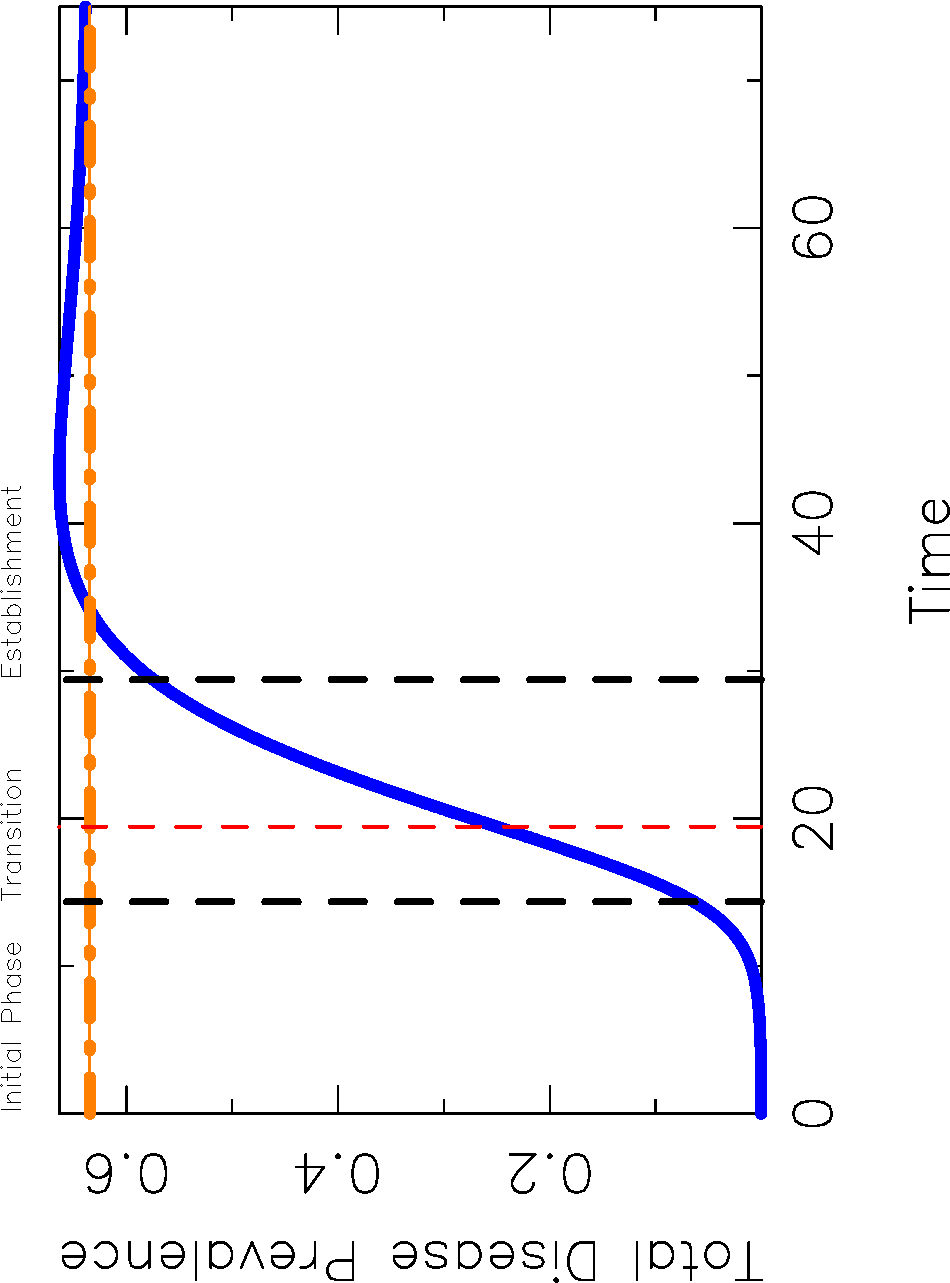
\includegraphics[scale=0.6,angle=270]{Sigmoidal_Curve.pdf}
\caption{Temporal evolution of model HIV total prevalence when using constant parameters (see column $V$ in Table \ref{T1:Parameter_Values}). The two vertical broken black lines define the three different phases as explained in the main text. The vertical broken red line defines the turning point. Since parameters are kept constant, the system reaches an asymptotic stationary state (horizontal broken orange line). The initial condition corresponds to a population with 10 infected sexual workers in a total population of sexual workers of 1000 within a total adult population (men and women) of 100000.}
\label{Fig2:Sigmoidal}
\end{figure}

\subsection{Model validation with data from 2000 to 2016}
Due to the paucity of disease data \cite{Raberahona2020}, model validation was a challenging task. We used all the data available from 2000 to 2016 to search for parameter combinations able to yield temporal trajectories in agreement with the few disease data at hand (see Fig \ref{Fig_Antsiranana_Fitted-vs-Extrapolated}), but the rich demographic information found in annual life tables from that period. The process of model assessment and validation was done in three different phases: (1) the simple demographic model ---see Eqs (\ref{Eq:Demography_S})---, (2) the expanded demographic model ---see Eqs (\ref{Eq:Demography_0})---, and, finally, (3) the full disease transmission model. Parameters distributions consistent with both demographic and disease data showed that model parameter values were further constrained by population and disease data over the studied period  (see Supp Mat for details). 
\smallskip

 \subsection{Model projections up to 2033}
The ensemble of parametric configurations providing good fit to data (see Table \ref{T2:Parameter_Values}) up to 2016 was then used to project the evolution of the disease up to 2033. The numerical integration of the full system requires annual time-dependent parameters, this is, future recruitment and mortality rates ($F_X$, $F_Y$, $\delta_X$, and $\delta_Y$) from 2016 to 2033. These were extrapolated from the same demographic life tables under the assumption that mortality and fertility rates maintain the trends observed between 2000 and 2016. This procedure yielded expected annual rates ($\delta_X$,  $\delta_Y$, $F_X$ and $F_Y$) up to 2033 (see Supplementary Material). 
\smallskip

Projected trajectories for a number of output variables can be calculated for every city (see Fig \ref{Fig:Infected_Trends_Extrapolated}). These trajectories all start with the same initial condition. The initial state is defined by the number of individuals in each disease phase ($S$, $I$, $L$, and $D$) in 2000 and prescribed according to available population data of urban populations along with the fact of a more than plausible early HIV introduction at very low numbers back in 2000. Importantly, our approach allows to compare the likelihood of different introduction years from 2000 on. Until approximately 2005, this likelihood is roughly the same, and then continuously drops down until the present (see Supp Mat, Fig D5). Although we cannot reliably say whether disease introduction was before 2000 or not, we can confidently conclude that introduction years later than 2004 become less and less plausible. Later introductions are less likely to reasonably provide the prevalence levels already observed across cities in 2012 and 2016. In any case, since our conclusions are robust to consider introduction years between 2000 and 2004, here we only reported results starting at 2000, under the assumption that the disease was already present, but at a very low prevalence, back then. 
\smallskip

In spite of the paucity of disease time series data and the uncertainty generated by the different parameter combinations, our model predicts a sharp increase in prevalence values around 2020 until reaching steady values over 2030. This pattern is consistent across cities. In Fig. \ref{Fig:Infected_Trends_Extrapolated}, for comparison, we only show results on prevalence across the different population groups for 5 important cities in Madagascar (see Supplementary Material for more details). Projected disease prevalence is shown here in terms of the distribution values across parametric configurations in a percentile manner, this is, instead of presenting the temporal evolution for each parameter combination in green (as in the left panels of Fig \ref{Fig_Antsiranana_Fitted-vs-Extrapolated}), here we show percentile levels 0.1, 0.5, and 0.9. This means that 80 \% of the solutions fall within this envelope. First column panels show, for instance, an increase of disease prevalence within the SW key population jumping from average values of 0.01 before 2015 to values as high as 0.6 after 2030, while overall prevalence in the total population stabilize around values from 0.2 to 0.3. We recall here that overall prevalence is given as a fraction of total adult population in every city. Finally, we visually show a summary of projected prevalence in 2033 in the general populations across cities over a map (see Fig \ref{Fig:Map}), and the turning-point year distributions for the ensemble of parametric configurations (see Fig. \ref{Fig_Turning_Points}).
\smallskip

% % % % % % % % % % % %   F I G U R E   H Y P O T H E S I S   % % % % % % % % % % % % % % % % % % % % % 
\begin{figure}[t]
	\centering
	\vspace{0.5cm}
	\begin{minipage}{0.47\textwidth}
		\centering
		\includegraphics[angle=0,width=1.0\textwidth]{Antsiranana_3Plots_Fitting.pdf}
		\subcaption[first caption.]{Model fit}\label{Neurona}	
	\end{minipage}%
	\hspace{0.01\textwidth}
	\begin{minipage}{0.47\textwidth}
		\centering
		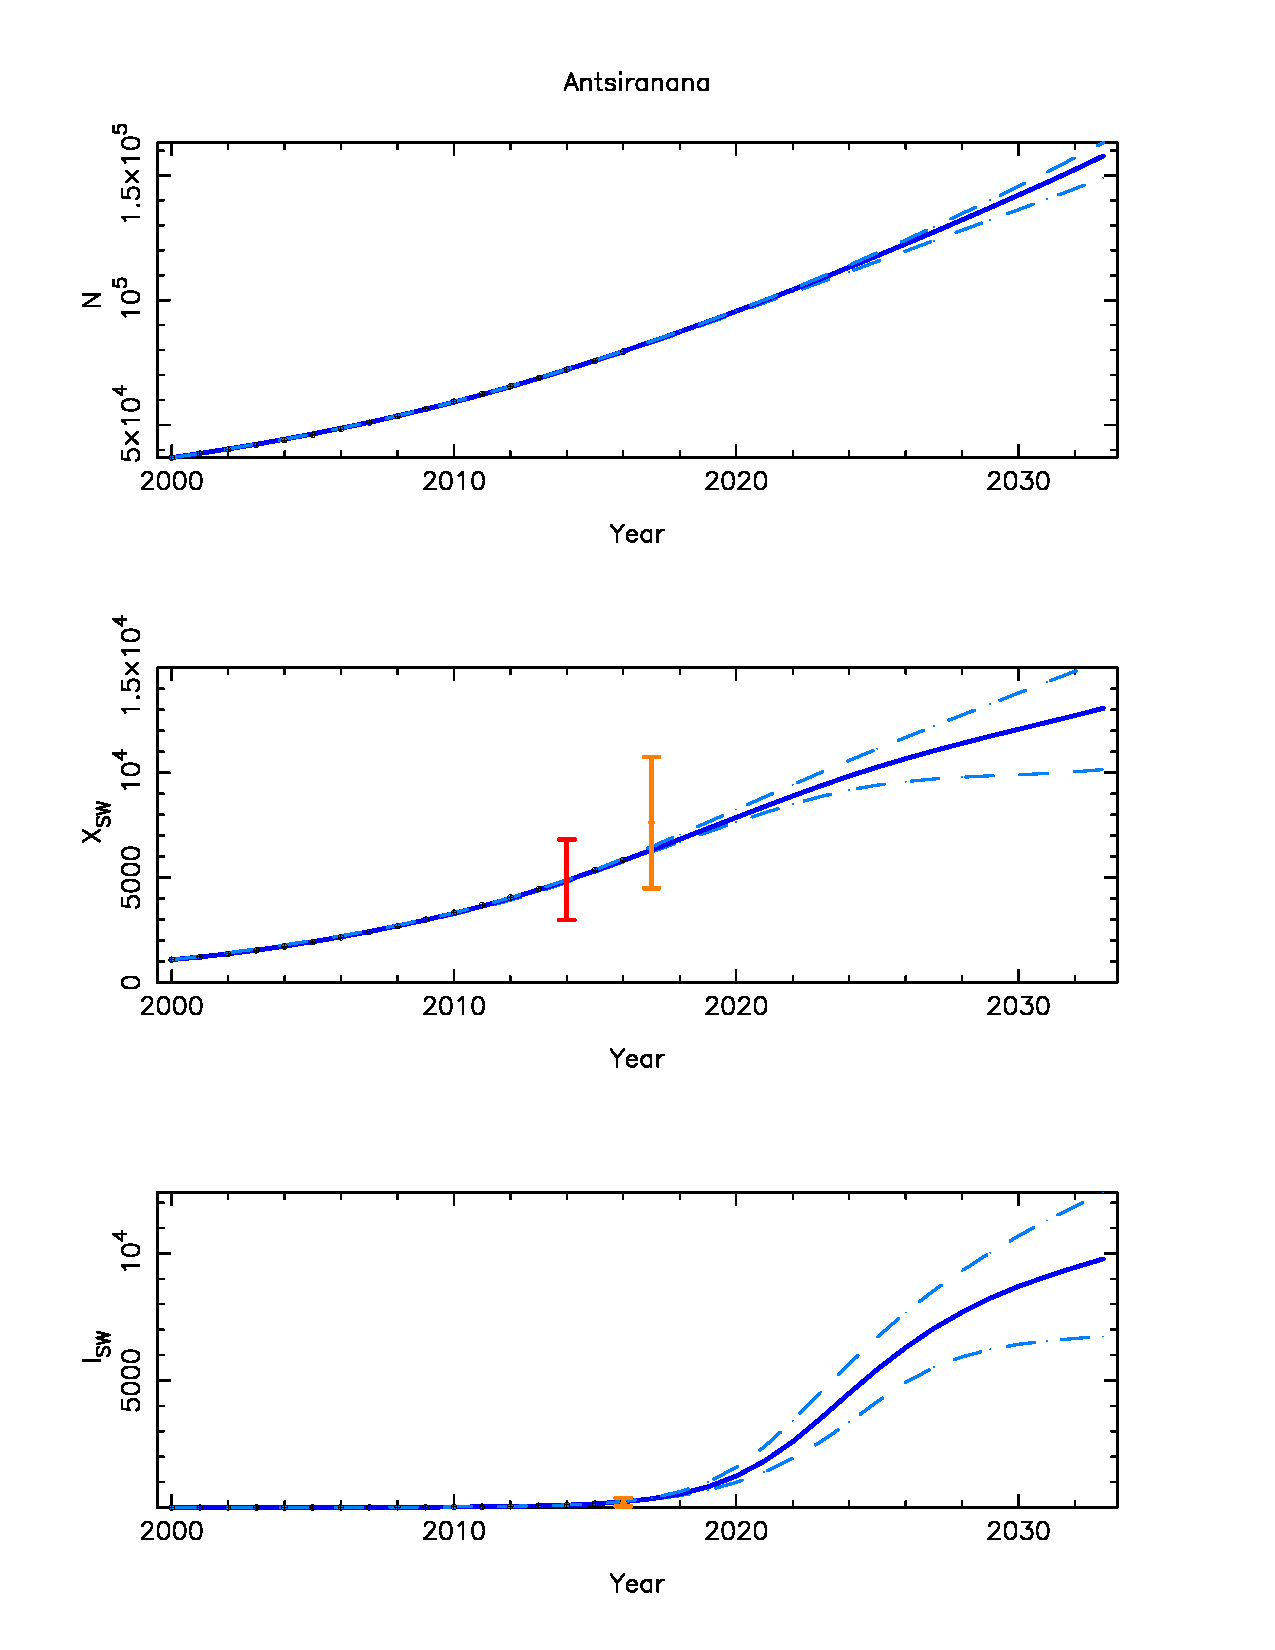
\includegraphics[angle=0,width=1.0\textwidth]{Antsiranana_3Plots_Projected.pdf}
		\subcaption[second caption.]{Future projection}\label{Volerrab}
	\end{minipage}
	
	\caption{Model fit and projected trends in Antsiranana. Here we show the model projections up to year 2033 calculated (b) for a number of parameter combinations that provide a good fit to data for the period 2000-2016 (a). Similar projections are obtained for other cities (see Supp Mat). Each parameter combination produces a single deterministic trajectory, which has been represented in green in (a). The ensemble of trajectories is used to calculate percentile values. Upper and lower broken lines represent the 90\% and 10\% percentile values, respectively. The thicker line in the middle represents 50\% percentile values. Pseudo-data for the period between 2000 and 2016 are represented by circles. They have been generated under the sigmoidal hypothesis to be compatible with the demographic expansion in Madagascar in this period (see Supp Mat). True data are highlighted with error bars representing confidence intervals (see years 2014 and 2017 in middle and lower right panels). $N$, adult population; $X_{SW}$, female sexual worker population; $I_{SW}$, infected individuals within the sexual worker population.}
    \vspace{-1.0cm}
    \label{Fig_Antsiranana_Fitted-vs-Extrapolated}
\end{figure} 
% % % % % % % % % % % % % % % % % % % % % % % % % % % % % % % % % % % % % % % % % % % % % % % % % % % % %
% \begin{figure}
% %\animategraphics[width=\linewidth,angle=270]{10}{cityParameters}{}{}
% 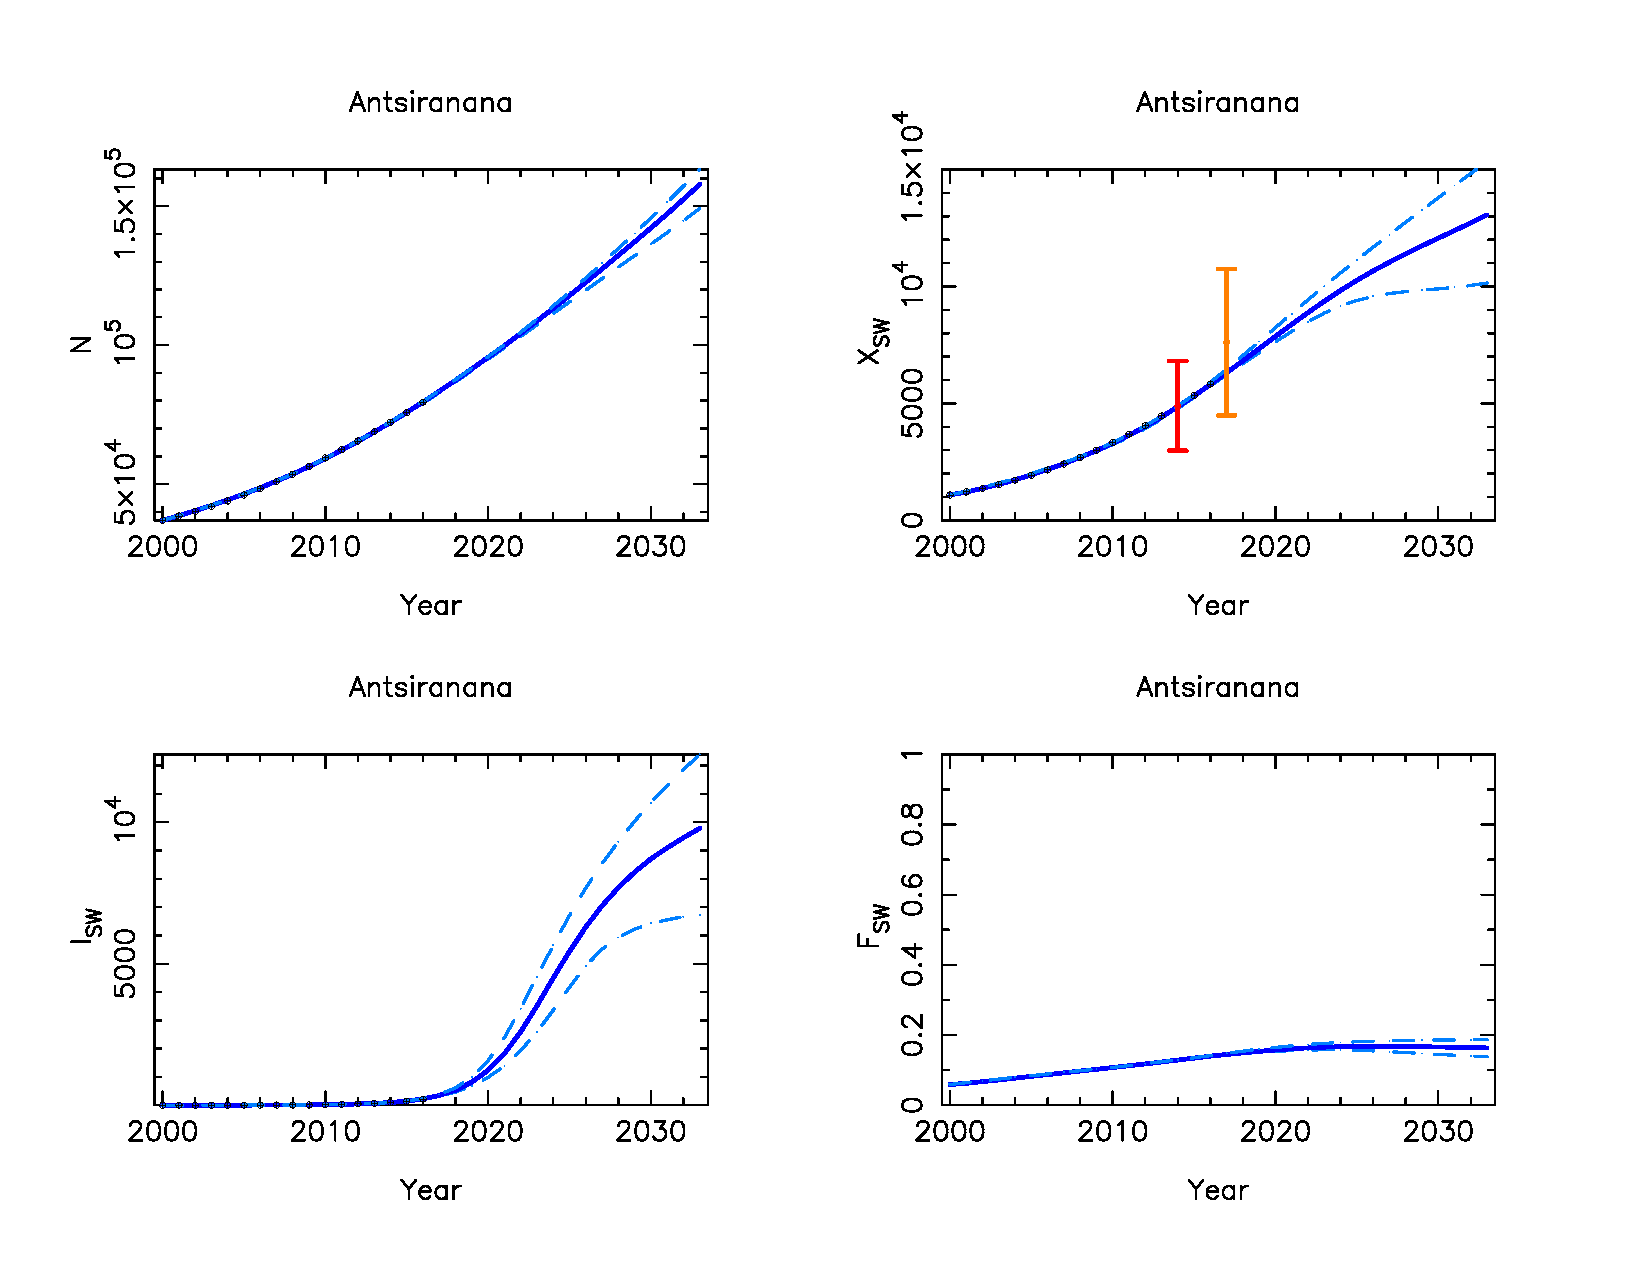
\includegraphics[width=\linewidth,angle=0]{Percentiles_Antsiranana.pdf}
% \caption{Projected trends in Antsiranana. Here we show the model projections up to year 2033 calculated for a number of parameter combinations that provide a good fit to data for the period 2000-2016. Similar projections are obtained for other cities (see Supp Mat). Each parameter combination produces a single deterministic trajectory. The ensemble of trajectories is used to calculate percentile values. Upper and lower broken lines represent the 90\% and 10\% percentile values, respectively. The thicker line in the middle represents 50\% percentile values. Data for the period between 2000 and 2016 are represented by circles, and generated under the same hypothesis, as in Fig \ref{Fig_Antananarivo_F_SW}. True data are highlighted with error bars representing confidence intervals (see years 2014 and 2017 in upper right panel). $N$, adult population; $X_{SW}$, female sexual worker population; $I_{SW}$, infected individuals within the sexual worker population, and $F_{SW}$, the sexual worker population fraction.}
% \label{Fig_Antsiranana_Extrapolated}
% \end{figure}

\begin{figure}
%\animategraphics[width=\linewidth,angle=0]{10}{cityParameters}{}{}
\vspace{-1.0cm}
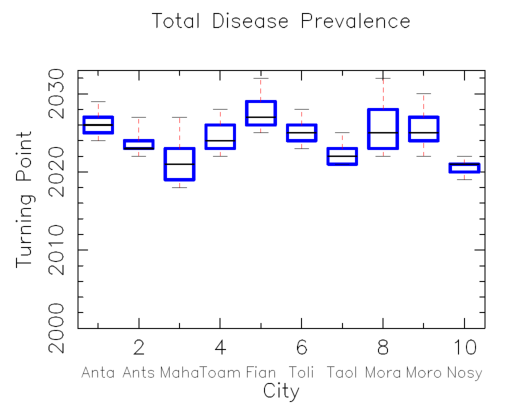
\includegraphics[width=\linewidth,angle=0]{boxplot-Total-Prevalence-Sigmoidal.pdf}
\caption{Turning points calculated for the projected prevalence within the general population in the 10 cities. Box plots represent distributions across the parameter configurations that provided a good fit to data for the period 2000-2016.}
\label{Fig_Turning_Points}
\end{figure}

\begin{figure}
%\animategraphics[width=\linewidth,angle=270]{10}{cityParameters}{}{}
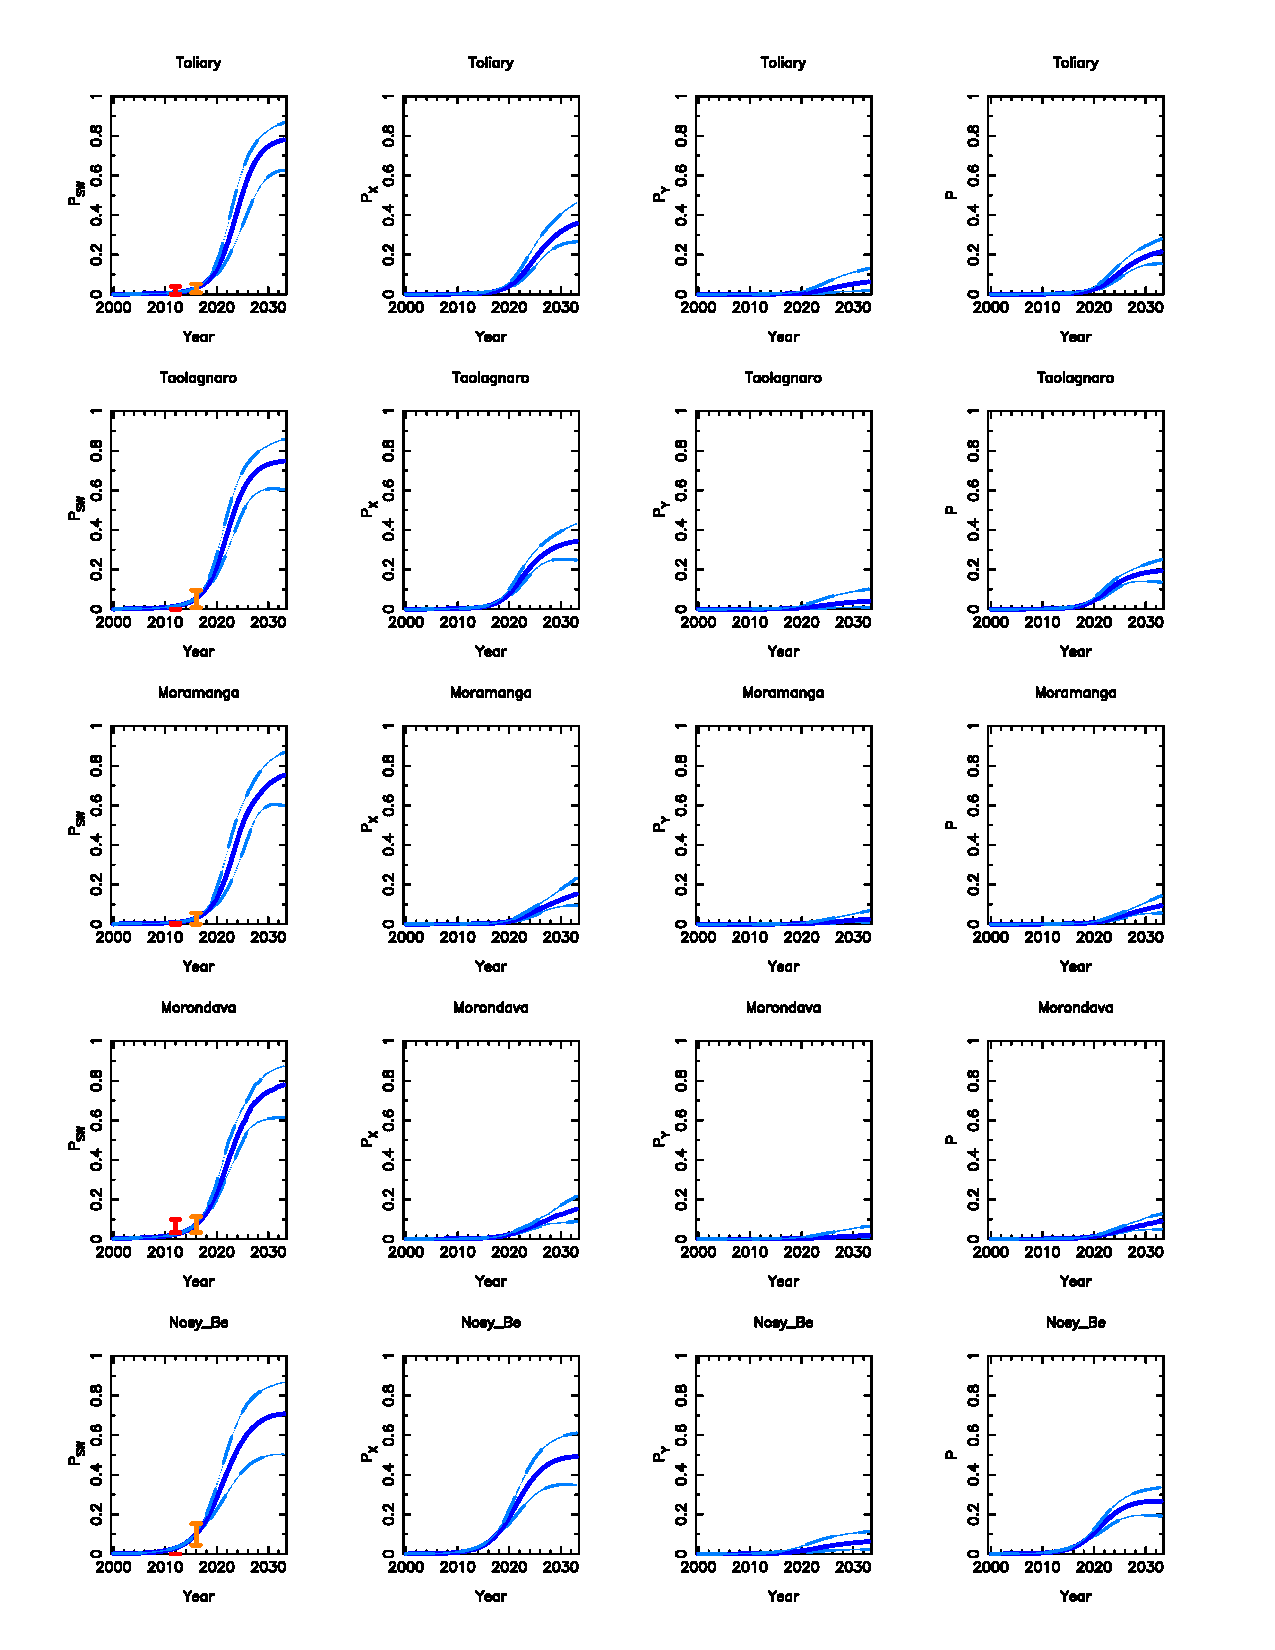
\includegraphics[width=\linewidth,angle=0]{Percentiles_Prevalence_10_Cities_B_Corrected.pdf}
\vspace{-1.0cm}
\caption{Predicted prevalence trends across 5 cities in Madagascar. True observed data are highlighted with error  bars representing confidence intervals for 2012 and 2016 (see panels in first column). Prevalence for the SW ($P_{SW}$), overall female ($P_X$), male ($P_Y$), and overall adult ($P$) populations are represented in columns 1 to 4, respectively. So the last column plots show total prevalence within the adult population.}
\label{Fig:Infected_Trends_Extrapolated}
\end{figure}

\section{Discussion}
 The underlying question that motivated this work was why Madagascar, in contrast with neighboring African countries, does not show a generalized epidemic profile yet. From our model-based analysis alone, we cannot come to a conclusive answer, but our work may help support some hypotheses and draft future scenarios. In this regard, our model suggests that the tipping point towards a generalized epidemics might have been delayed through the widespread practice of circumcision although the effect is too slight to prevent disease expansion (see Figs B2 and E7 in Supp Mat), and/or a late/slow introduction of HIV in the island compared to continental Africa. However, some authors pointed out that circumcision, over a certain threshold of HIV prevalence among SW’s has not a substantial effect towards HIV prevention at population level \cite{Talbott2007}. If true, given the observed trends among SW's in recent years (Fig \ref{Fig:Map}), the potential protective effect of circumcision may have already vanished in Madagascar. Other damping factors could have been a rather low population density and lower mobility \cite{Raberahona2020}. In any case, the estimated tipping points are close or may have been overcome in different locations (see Figure \ref{Fig_Turning_Points}). 
 \smallskip
    
The main strength of our model is the inclusion of different infectiousness levels through the stages of the natural history of a HIV infection, shaped by behavioural risk factors. More precisely, our approach considered (1) a straightforward integration of demographic life table data, (2) the differential transmission male-to-female risk and vice versa, which allows to explore the effect of male circumcision, (3) three stages of disease progression since acquiring the infection if untreated (acute, chronic, and AIDS, see Fig \ref{Fig:1}) , and (4) known behavioral risk factors associated with HIV acquisition. Likewise, our model allows us to analyze the effect of early infected and acute infectious individuals on the early stages of epidemic expansion. This effect could have been very important in Madagascar at the beginning of the studied period. The relative contribution of acute infections at the early stages of disease expansion has been estimated much higher than the role they play in disease maintenance once the infection is well-established in the population \cite{Fiebig2003}. Recent modeling approaches, although simpler in the treatment of the female group, take also into account ARV coverage \cite{Omondi2018,Omondi2019}, but treatment coverage in Madagascar is   very low according to official reports(8 \% \citet{UNAIDS2019}) and was not included. 
\smallskip
 	  
Main parameters of HIV transmission established by previous observational studies lie within the bounds of our model estimations, which supports the robustness of our model. $R_0$ values in 2000, where prevalence was thought to be very low, and which depends on most model parameters through Eq (\ref{eq:R_0}) vary between 3 and 8 across the different cities (Table \ref{T2:Parameter_Values}). This is in good agreement with  observational (not-model based) estimations \cite{Nsubuga2014}. However, our estimates of $R_0$ may be a little inflated because they are calculated under the assumption of random sexual contacts between the different groups \cite{Diekmann2010}. Moreover, these values are particularly useful for relative comparisons, and to elucidate which model parameters have the highest influence on disease propagation just after HIV introduction. They represent highest bounds, as it is known that in general contact heterogeneity \cite{Britton2020}, and non-random sexual mixing, for instance, sequential monogamy \cite{Hollingsworth2008}, commonly slows down disease propagation, but precise estimations of the prevalence of these sexual behaviour factors in Madagascar are not available. Our estimation procedure potentially also informs about male sexual preferences for young (Adolescent Girls and Young Women, AGYW, 15-24 years old) or adult women (see parameters $f_W$ and $f_0$ in Table \ref{T2:Parameter_Values}, and also Fig F8, Supp Mat). 
\smallskip

Our HIV compartmental model was framed by the central consideration of commercial sex as a driver of HIV epidemic. The number of HIV-positive SW's has been recognized as the main driver leading to a generalized epidemic in countries \cite{Talbott2007}, but has been overlooked by previous modelling work \cite{Kim2014,Omondi2018,Mukandarive2007}. Furthermore, we expanded the classical concept of SW (women that recognize themselves as SW and for whom sexual services are the main source of incomes) with the inclusion of TS (occasional sexual intercourse in exchange for any material or non-material benefit other than money). TS has been underscored as a risky factor for HIV expansion \cite{Wamoyi2016}, and it is specially prevalent among AGYW. A disproportionate fraction of sexual encounters between males and younger females (intercourse mixing age heterogeneity)  has been repeatedly noticed as a risk factor of HIV acquisition for AGYW on itself \cite{Stoner2020}  , and through associated risky behaviours to this kind of relationships, such as concurrency and inconsistent use of condoms \cite{Anderson1992,Maughan-Brown2016,George2019a,Evans2017}. Thereby, AGYW is now considered as a truly KP in most Sub-Saharan countries \cite{Dellar2016}, and this vulnerability may be mediated by the practice of TS and the male sexual preference for younger women. In countries with well established HIV epidemics, this subpopulation may have six or seven fold risk of HIV acquisition compared to male of the same age  \cite{Leclerc2008,Dellar2016}. In Madagascar, all of these factors and behaviors have been reported as highly prevalent \cite{Raberahona2020}. Therefore, our model allows to consider, as well, the critical interaction between primary HIV infection (a short but highly infectious period) and concurrency \cite{Eaton2011,Mah2011,Kim2010,Goodreau2012}, and other risky factors \cite{Hollingsworth2008}, which are associated to the described pattern of AGYW sexual behaviours. To the best of our knowledge, previous HIV compartmental models do not consider these critical interactions. As a consequence, their predictions of epidemic dynamics may be, in a certain extend, inaccurate.
\smallskip

Our estimated prevalence trajectories are invariably sigmoid-like curves with three typical phases from introduction to establishment (see Fig \ref{Fig:Infected_Trends_Extrapolated}). The initial phase may last about 15 to 25 years, characterized by low but slightly increasing prevalence. This phase quickly gives rise to a sharp transition from low to high prevalence values, which lasts about 10 years (intermediate phase). Full disease establishment is only attained after about 35 to 55 years since disease introduction. These curves show turning points between years 2020 and 2022 (see Fig \ref{Fig_Turning_Points}). Consequently, our results strongly suggest that some cities are very close or even have surpassed the tipping point. Therefore, unless a sustained action is taken, future HIV prevalence in Madagascar for next decade (2030s) may be similar to other HIV/AIDS highly hit countries from the Southern African region (see Fig \ref{Fig:Map}, between 20-30 \% \cite{Epstein2011}). 
\smallskip

In the range of our parameter estimates, our model invariably predicts that the SW population is the first to take off in the trajectory towards disease establishment and the one that reaches higher prevalence values (Fig. \ref{Fig:Infected_Trends_Extrapolated}). This is in full agreement with previous work \cite{Bershteyn2013}. SW’s HIV prevalence may be the startup of the HIV introduction into GP through bridge populations (clients), and TS mainly practiced by young women (AGYW). An intercourse mixing-age model and associted risky behaviors could play a crucial role in the spread and maintenance of the epidemics once HIV prevalence has reached a certain threshold among GP (see Fig \ref{Fig2:Discussion}). Then, at certain stage, the HIV epidemics may evolve independently from the number of HIV positive SW's \cite{Bershteyn2013}. It is of note that the widespread presence of SW and TS is strongly influenced by underlying socio-economical factors, since they are both driven by financial insecurity and poverty \cite{Ingabire2012,Fitzgerald-Husek2011}. TS and SW tend to increase if the economical situation is worsening. Moreover, Madagascar is a highly vulnerable low-income country, as it became clear during the 2009-2013 economical crisis. Consequently, our model may underestimate the speed of transition towards generalized epidemics if a major economical crisis occurs, as we expect for the current COVID-19 epidemic. In this sense, it is striking to observe that impact projections on HIV/AIDS epidemics of COVID-19 crisis focus on sustained provision of ARV drugs and HIV-services provision \cite{Jewell2020}, and obliterate other co-factors like the increasing vulnerability to HIV which is mostly female-gender dependent.
\smallskip

% These results underline that too general and unspecific estimations of disease incidence at national level may be misleading. The baseline data and our model estimates indicates that HIV epidemic in Madagascar is evolving following a patchwork pattern focused on major cities, but, as observed in other Sub-saharan countries, it is expected that from there HIV would slowly penetrate rural areas in the inner country (ref. DRC).  Therefore, each region or city should require a tailored intervention with different priorities. 
\smallskip

\begin{figure}
\centering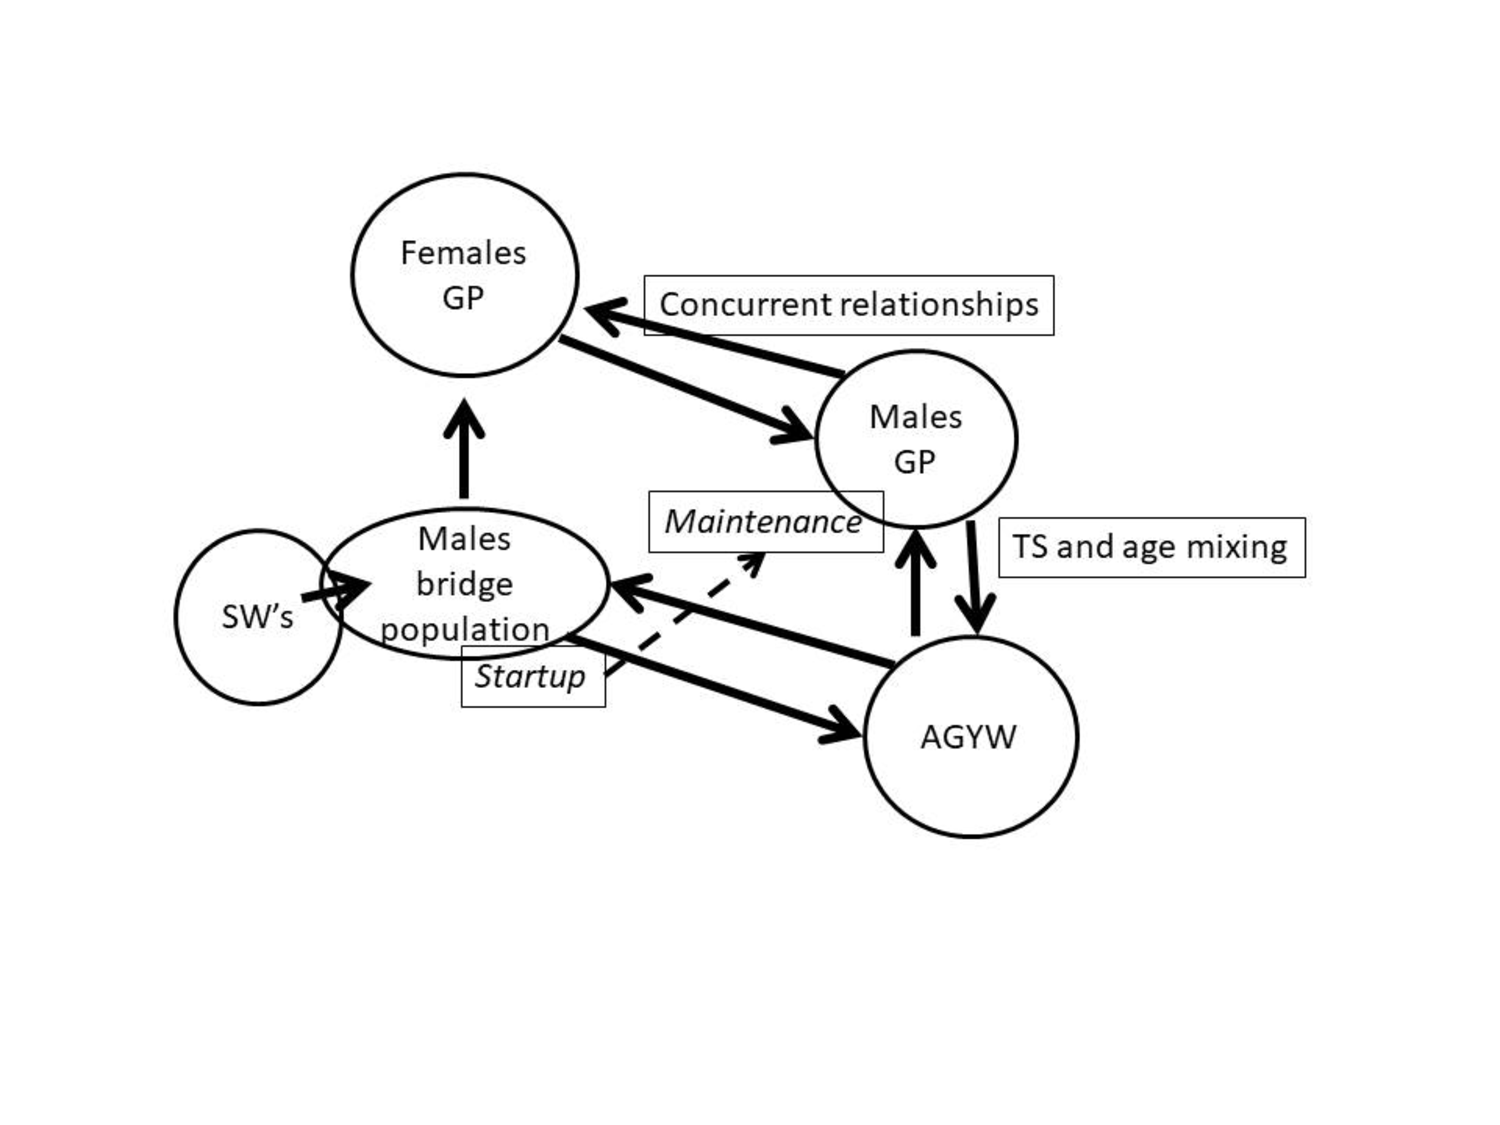
\includegraphics[width=1.0\linewidth,angle=0]{Figure_discussion.pdf}
\caption{In this figure we show the conceptual model of HIV progression from concentrated epidemic to generalized and self-maintained epidemic in countries with the socio-behavioural characteristics of Madagascar. The start up of the epidemic is characterized by a long-lasting and steady increase of HIV prevalence among SW’s. HIV infection spills over to GP (adult females, AGYW and indirectly other GP males) through bridge population (SW clients). The intensity of this spill initial over is enhanced as prevalence among SW increases in positive feedback manner. Once a certain threshold in GP has been reached, prevalence/incidence in GP may be self-sustained and tend to increase through high risk intercourse between AGYW and older adults. This threshold may be reached sooner depending on the prevalence of age disparate relationships, concurrency and inconsistent use of condoms. Transactional sex may be the main mediator of such risk factors.}
\label{Fig2:Discussion}
\end{figure}

As any modelling exercise, our work has also limitations. Firstly, there is little information available on the women distribution in the different key groups (SW and TS). Specific hypotheses controlling this distribution are implicitly assumed in the set of $\sigma$ model parameters (see Supp Mat). Secondly, there is no direct data on age-disparity sexual relationships in Madagascar. These information gaps should be urgently filled in order to set up better disease control strategies and to obtain better and more accurate projections. An intriguing point in the data available is the significant decrease of SW's observed between the 2014 and 2017, particularly in some cities (see Table \ref{Table:Madagascar_Cities}). Besides the possible bias of the estimated key populations in both years \cite{Raberahona2020}, it could be argued that sex working has declined thanks to the slow recovery of the economy in Madagascar after 2013.  Moreover, it is clear that further model development is also required. A well-known risk factor increasing HIV transmission not considered here is the concurrency with other the Sexual Transmitted Infections (STI), which have a catalytic effect on HIV transmission \cite{Torrone2018}. The consideration of this factor is hindered by the lack of reliable population-level data on STI's prevalence in Madagascar, even though some studies have reported extremely high prevalence of STI's among SW's and GP \cite{Raberahona2020} as in other African countries \cite{Torrone2018}. Our model does not considered either other KP's, like MSM and IDU, but their role in the generalization of an epidemics could not be excluded, as it has been observed elsewhere \cite{Celentano1998}. Furthermore, the role of IDU has been underscored in Sub-Saharan Africa \cite{Asher2013}, and this represents an increasing population in Madagascar. The bridge between these KP’s and GP through bisexual intercourses (MSM), and sex working (IDU), should be further explored. Finally, future models of this kind should also take into account mobility between localities. At this stage, our model does not consider the mobility of risky populations (SW's) between cities following tourist seasons, as it has been reported in Mahajanga and Nosy-be (the two cities with higher HIV prevalence among SW's) \cite{Raberahona2020}. This dynamics may foster even more the diffusion of HIV over other parts of the country. 
\smallskip

\begin{figure}
\centering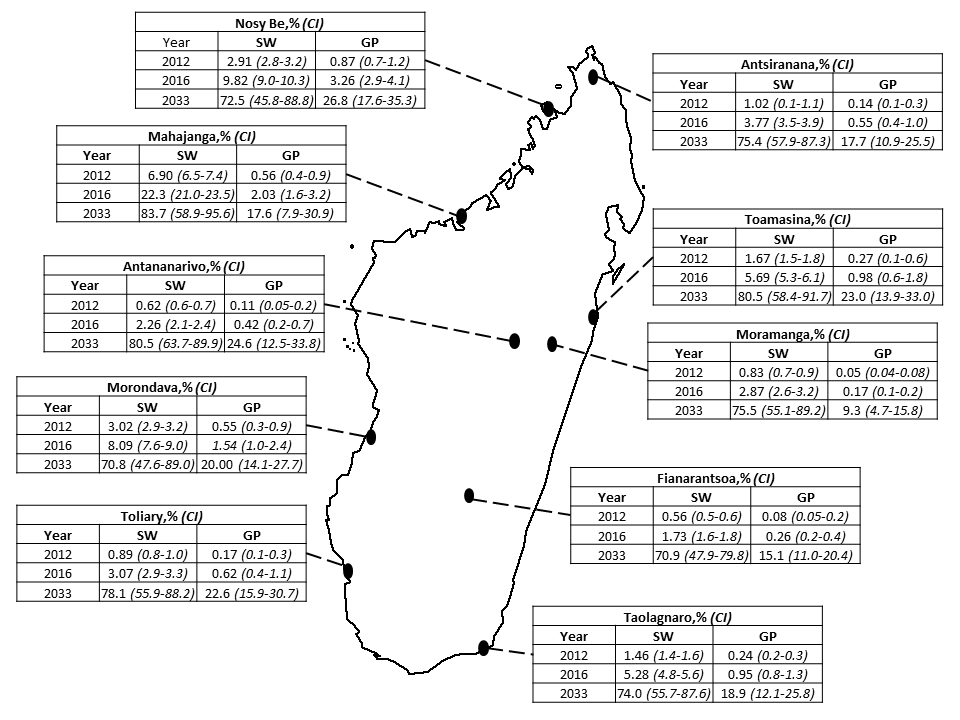
\includegraphics[width=1.0\linewidth,angle=0]{Figure 1_modelling.png}
\caption{HIV prevance levels both in the general (GP) and in the SW population for the two years for which surveyed data existed (2012 and 2016) along with model prediction for 2033.}
\label{Fig:Map}
\end{figure}

Even admitting that our model is based on simplifying assumptions, given our projections it is worrisome to see that Madagascar shows some of the poorest HIV response indicators in the world (only 8\% of PLWHIV are estimated to be under follow-up \cite{UNAIDS2019}). A key question remains to be answered once more accurate data are available from Madagascar: are we still in time to avoid a generalized epidemics in Madagascar? As a conclusion, given the plausibility of the worse case scenario we outline here, it is important to set up observational studies on HIV prevalence/incidence and risky factors, alongside the implementation of robust preventive measures focused on monitoring and identifying hot-spots and vulnerable key populations (SW and AGYW). These results would be extremely helpful for a better focused and monitored HIV prevention response and provide guidance to health authorities. The successes observed in India or Thailand \cite{IndiaReport2016,Celentano1998}, where a generalized epidemics was foreseen but was avoided by a robust and targeted response, is very encouraging. We hope that our model will become an additional tool for directing the HIV/AIDS response in Madagascar, and a source of inspiration to develop control strategies in other countries as well. 

%% The Appendices part is started with the command \appendix;
%% appendix sections are then done as normal sections
%% 
%% References
%%
%% Following citation commands can be used in the body text:
%% Usage of \cite is as follows:
%%   \cite{key}          ==>>  [#]
%%   \cite[chap. 2]{key} ==>>  [#, chap. 2]
%%   \citet{key}         ==>>  Author [#]
%% References with bibTeX database:
\newpage
\bibliographystyle{model1-num-names}
\bibliography{sample.bib,Madagascar.bib}

%% Authors are advised to submit their bibtex database files. They are
%% requested to list a bibtex style file in the manuscript if they do
%% not want to use model1-num-names.bst.

%% References without bibTeX database:
% \begin{thebibliography}{00}
%% \bibitem must have the following form:
%%   \bibitem{key}...
%%
% \bibitem{}

% \end{thebibliography}
\end{document}

%%
%% End of file `elsarticle-template-1-num.tex'.